\newpage
\appendix

% \begin{itemize}
%     % \item model architecture full details (with Linear Layers, LN, normalizations, silu etc). Can be in the same section as the pytorch-stype LaCT pesudo code for our TTT layer. => init.
%     % \item pytorch style pesudcode code.  
%     \item context parallelism pesudocode code.
%     \item In supp, add a detailed equation wise comparison with origina ttt. 
%     \item The detailed model and experiment setting for each experiment  -> LVSM(Hao), Video, Language.  Model.  Training. Eval. Baseline.  [Numbers for each figures]. 
%     \item mamba2 video
%     % \item flops analysis for fast weight and also muon.  cost effectiveness analysis of muon.  $15 d^3$ -> $18 n d^2$
%     \item video results and sampling. GSO 1K res rendering, DL3DV rendering at all number of views. Some tables for videos. 
% \end{itemize}


% \hao{Need to provide the GPU numbers; this is a checklist answer that I selected Yes.}





\section{\methodname{} Model Implementation Details }
\label{sec:appen_lact_details}

\begin{algorithm}[p]
\caption{Large Chunk Test-Time Training Layer Pseudocode}\label{alg:full_lact_layer}
\newcommand{\hlbox}[1]{%
  \fboxsep=1.2pt\hspace*{-\fboxsep}\colorbox{blue!10}{\detokenize{#1}}%
}
\lstset{style=mocov3}
\begin{lstlisting}[
    language=python,
    escapechar=@,
    label=code:lact_full]
    def apply_fw(fast_weight, q):
        w1, w2, w3 = fast_weight
        hidden = silu(matmul(q, w1)) * matmul(q, w3) # [b, l, dh] = [b, l, d] x [b, d, dh]
        return matmul(hidden, w2)
        
    def update(fast_weight, k, v, lr, use_muon=True):
        """
        Fast-weight update for a SwiGLU MLP using chunk of tensors. 
        Args:
            fast_weight : tuple(w1, w2, w3) with shapes: w1, w3: [b, d, dh]; w2: [b, dh, d]
            k, v        : key / value tensor of shape [b, l, d]
            lr:         : per-token learaning rates of shape [b, l, 3] -> (lr1, lr2, lr3)
            use_muon    : weather to apply Muon to orthogonalize the update
        Note:
            The head dimension for input tensors k, v, lr are assumed to be merged into the batch dimension. This is not necessary, but simplifies shape annotation in this pseudocode.
        """
        # Forward with k:
        gate_before_act = matmul(k, w1) # [b, l, dh] = [b, l, d] x [b, d, dh]
        hidden_before_gate = matmul(k, w3) # [b, l, dh] = [b, l, d] x [b, d, dh]
        hidden = silu(gate_before_act) * hidden_before_gate
        
        # Backward:
        dhidden = matmul(v, w2.transpose(-1, -2)) # [b, l, dh] = [b, l, d] x [b, d, dh]
        dhidden_before_gate = dhidden * silu(gate_before_act)
        dgate = dhidden * hidden_before_gate
        dgate_before_act = silu_backprop(dgate, gate_before_act)

        # Compute gradients: 
        w2.grad = -matmul(hidden.transpose(-1, -2), v * lr2) # [b, dh, d] = [b, dh, l] x [b, l, d]
        # [b, d, dh] = [b, d, l] x [b, l, dh]
        w1.grad = -matmul((k * lr1).transpose(-1, -2), dgate_before_act)
        w3.grad = -matmul((k * lr3).transpose(-1, -2), dhidden_before_gate)

        # Weight update
        if use_muon:
            for w in fast_weight:
                w.grad = zeropower_via_newtonschulz5(w.grad)
        for w in fast_weight:
            w = (w - w.grad) / (w - w.grad).norm(dim=1) * w.norm(dim=1)
        return fast_weight

    def silu_backprop(dy, x):
        sigma = sigmoid(x)
        return dy * sigma * (1 + x * (1 - sigma))

    #################################### MultiHead LaCT layer ####################################
    # x: input sequence [b, l, d], b is the batch dim, l is length, d is model dimension
    # fast_weight: tuple of initial fast weights-(w1, w2, w3); w1, w3 of shape [nh, d, dh], w2: [nh, dh, d]
    # ttt_config: list of (operation, begin, end) tuples
    qkv = silu(LinearQKV(x)) # [b, l, d * 3]
    qkv = rearrange(qkv, `b l (nh hd) -> (b nh) l hd`, nh=num_heads).split(3) # merge heads into batch dim
    q, k = q / q.norm(-1), k / k.norm(-1)
    lr = softplus(LinearLR(x) + const_lr_bias) # [b, l, 3 * num_heads]
    lr = rearrange(lr, `b l (nh 3) -> (b nh) l 3`, nh=num_heads)
    fast_weight = repeat(fast_weight, dim=0, repeat=b) # [nh, ...] -> [b * nh, ...]
    
    o = zeros_like(v) # [b * nh, l, hd]
    for mode, begin, end in ttt_config:
      qi, ki, vi, lri = q[:, begin:end], k[:, begin:end], v[:, begin:end],  lr[:, begin:end]
      
      if mode == "update_then_apply": # figure-3(a, b) bidirectional attention
        fast_weight = update(fast_weight, ki, vi, lri, use_muon)
        o[:, begin: end] = apply_fw(fast_weight, qi)
        
      elif mode == "apply_then_update": # figure-3(b) shifted block-wise causal
        o[:, begin: end] = apply_fw(fast_weight, qi)
        fast_weight = update(fast_weight, ki, vi, lri, use_muon)

      elif mode == "update_only":
        fast_weight = update(fast_weight, ki, vi, lri, use_muon)
      
      elif mode == "apply_only":
        o[:, begin: end] = apply_fw(fast_weight, qi)

    o = RMSNorm(o) # per-head norm
    o = LinearOutput(rearrange(o, `(b nh) l hd -> b l (nh hd)`, nh=num_heads))
    return o
\end{lstlisting}
\end{algorithm}




\begin{algorithm}[t]

\caption{LaCT Layer with In-Layer Hybrid Window Attention Pseudocode}\label{alg:lact_hybrid}
\newcommand{\hlbox}[1]{%
  \fboxsep=1.2pt\hspace*{-\fboxsep}\colorbox{blue!10}{\detokenize{#1}}%
}
\lstset{style=mocov3}
\begin{lstlisting}[
    language=python,
    escapechar=@,
    label=code:gslrm]
    # Input: 
    # x: input sequence [b, l, d], b is the batch dim, l is length, d is model dimension
    # fast_weight: tuple of initial fast weights-(w1, w2, w3); w1, w3 of shape [d, dh], w2 of shape [dh, d]
    # ttt_config: list of (operation, begin, end) tuples

    q, k, v = LinearQKV(x).split(3)
    
    #### Local quadratic-cost window attention
    attn_q = q * learnable_q_scale + learnable_q_offset # per-channel rescale and shift
    attn_k = k * learnable_k_scale + learnable_k_offset # per-channel rescale and shift
    attn_o = local_softmax_multihead_attn(attn_q, attn_k, v, attn_mask)
    
    #### large chunk test-time training for long memory
    q, k = rearrange(q, k, `b l (nh hd) -> (b nh) l hd`, nh=num_heads)
    q, k = silu(q), silu(k)
    q, k = q / q.norm(-1), k / k.norm(-1)
    lr = softplus(LinearLR(x)) # [b, l, 3 * num_heads]
    lr = rearrange(lr, `b l (nh 3) -> (b nh) l 3`, nh=num_heads)

    # Perform update and apply_fw operations iteratively over chunks of tokens.
    lact_o = lact(fast_weight, q, k, v, lr, ttt_config)
    lact_o = RMSNorm(lact_o)
    
    scale_per_head = rearrange(silu(Linear(x)), `b l nh -> (b nh) l 1`, nh=num_heads)
    lact_o = lact_o * scale_per_head
    lact_o = rearrange(lact_o, `(b nh) l hd -> b l (nh hd)`, nh=num_heads)

    #### Merge attention results (shape: [b, l, d])
    o = attn_o + lact_o

    o = LinearOutput(o)

    return o
\end{lstlisting}
\end{algorithm}


% In our Large-Chunk TTT layer, we first take three Linear layers to convert the input to Query (Q), Key (K), and Value (V).  
% Then we use 
% We predict one learning rate for each token and each fast weight.
% chunk into we follow \hao{CITE} to  \tianyuan{I don't think we need a text description of the process?}




\paragraph{State Size calculation.} Motivated by recent progress in LLM, we adopt SwiGLU-MLP~\cite{shazeer2020glu} without bias terms as the fast-weight 
network. 
Our fast weights consists of three weight matrix $W = \{W_1, W_2, W_3\}$, and the forward pass of the fast weight model is:
\begin{equation}
f_W(x) = W_2 \left[ \mathrm{SiLU}(W_1 x) \circ (W_3 x) \right]
\label{eq:swiglu_supp}
\end{equation}
where $\circ$ is an elementwise multiplication. We define $\mathit{hd}$ as the head dimension, $\mathit{nh}$ as the number of heads, and the intermediate dimension of the SwiGLU-MLP as $\mathit{hd} \times r$, where $r$ is a scaling multiplier.When $r > 1$, the intermediate dimension surpasses the input head dimension, which is the current common practice in LLMs.  TThus, matrices $W_1, W_2 \in \mathbb{R}^{\mathit{hd} \times \mathit{hd}}$ and $W_3 \in \mathbb{R}^{\mathit{hd} \times \mathit{hd} \times r}$. Consequently, the total state size becomes $\mathit{nh} \times \mathit{hd} \times \mathit{hd} *r$.  Given that typically the total head dimension across all heads equals the model dimension $d$ (i.e., $\mathit{nh} \times \mathit{hd} = d$), the total state size simplifies to:
\begin{equation}
    \text{State Size} = \frac{d^2}{\mathit{nh}} * r.
    \label{eq:state_size}
\end{equation}
Therefore, we can increase the state size either by reducing the number of heads or by increasing the intermediate dimension multiplier.


\paragraph{FLOPs calculation.} When using then negative dot product loss as the online test-time training objectives, we don't need to compute the final results of $f_W(v)$. We only need to compute $W_1v, W_3v$ when running forward pass with keys $k$, thus there are two matmuls in the forward pass with keys.  When computing the gradients, there are four matmuls. And in the final forward pass the queries, there would be three matmuls. So the total FLOPs with $n$ tokens would be:
\begin{equation}
    \text{FLOPs} = 4n \frac{d^2}{\mathit{nh}}r +  8n \frac{d^2}{\mathit{nh}}r +  6n \frac{d^2}{\mathit{nh}}r  = 18n \frac{d^2}{\mathit{nh}}r = 6 * \text{State Size} 
\end{equation}

\paragraph{Model initializations.} We randomly initialize the linear layers using a standard deviation of 0.02. For the learnable initial fast weights, we initialize them with a standard deviation of $1.0 / \sqrt{\text{fan-in}}$. Specifically, in the SwiGLU FFN fast weights, the matrices $w_1$ and $w_3$ have their fan-in set as the head dimension, while the fan-in of $w_2$ is the intermediate dimension of the SwiGLU FFN fast weights. Additionally, when local window attention is incorporated within the \methodname{} layer, we introduce four extra learnable embeddings: two scales and two reshifts for queries and values. We initialize the scale embeddings as ones and the reshift embeddings as zeros.


\paragraph{Details of Muon.} Muon~\cite{jordan2024muon} is a recently proposed optimizer that orthogonalizes the matrix gradients during updates of matrix weights. It utilizes Newton-Schulz iterations to achieve orthogonalization. Given a matrix gradient $G$, Muon first normalizes it as $G_0 = G / |G|F$, then iteratively applies:
\begin{equation}
\mathbf{G}_k = a\mathbf{G}_{k-1} + b(\mathbf{G}_{k-1}\mathbf{G}_{k-1}^{\mathrm{T}})\mathbf{G}_{k-1} + c(\mathbf{G}_{k-1}\mathbf{G}_{k-1}^{\mathrm{T}})^2\mathbf{G}_{k-1},
\label{eq:muon_iteration}
\end{equation}
where the constants $a, b, c$ are carefully chosen for optimal convergence. Following the original implementation, we set $a=3.4445$, $b=-4.7750$, $c=2.0315$, and perform five iterations.

Each Muon iteration requires three matrix multiplications, resulting in a computational cost per fast weight head of $2 \mathit{hd}^3 r + 2 \mathit{hd}^3 + 2 \mathit{hd}^3 r = \mathit{hd}^3 (4r + 2)$ FLOPS. Hence, the total computation for five iterations across all fast weights is:
\begin{equation}
5 \times \mathit{nh} \times \mathit{hd}^3 \times (4r + 2).
\end{equation}

For the case where $r=1$ (head and intermediate dimensions are equal), the total computational cost simplifies to:
\begin{equation}
30 \times \mathit{nh} \times \mathit{hd}^3 = 30 \times \mathit{hd} \times \text{State Size}.
\end{equation}
This indicates that the computational overhead of Muon becomes less significant than computing token outputs only if the online chunk size exceeds $\frac{5}{3} \mathit{hd}$.


\paragraph{Rotation invariance.} Softmax attention and linear attention exhibit rotation invariance: rotating the queries and keys by the same rotation matrix does not alter the output. This property is also used in developing relative positional encodings, like RoPE~\cite{su2023roformer}. In contrast, our SwiGLU and Linear Fast Weight components do not possess this property.


\paragraph{Implementing momentum for test-time optimizers.}  \label{paragraph:momentum}
Muon uses momentum by default. Following Titans~\cite{behrouz2024titans}, we implement momentum in the test-time optimizer by predicting a scalar momentum $\beta_i$ from each token: 
\begin{equation}
    \beta_i = \sigma(\text{Linear}(\boldsymbol{x_i})), 
\end{equation}
where $\sigma$ is the sigmoid function.  This $\beta_i$ is then averaged over all tokens in the chunk, and the average momentum is applied as follows:
\begin{equation}
\begin{aligned}
    g \leftarrow&  \sum_i^b \eta_i \nabla_W \mathcal{L}(f_W(k_i), v_i), \\
    M \leftarrow&  M (\sum_i^b \beta_i / b) + g, \\
    W \leftarrow& \text{weight-update}(W, M),
\end{aligned}
\end{equation}
where the $\text{weight-update}$ can be simple subtraction followed by L2 normalization normalization (as in Equation~\ref{eq:fast_weight_normalization_nomuon}). or Muon update before subtraction (as in Equation~\ref{eq:fast_weight_normalization}).


\subsection{Pseudocode}
\label{sec:ttt_pseudocode}


See Algorithm~\ref{alg:full_lact_layer} for pseudocode of a full \methodname{} layer. 
For details on how to mix local window attention inside each layer with shared query, value, embedding, see Algorithm~\ref{alg:lact_hybrid} for pseudocode. 





\section{\methodname{} Architecture Details for N-Dimensional Data }
\label{sec:appen_model_arch}

\subsection{\methodname{} Architecture for Novel View Synthesis}
\label{sec:appen_nvs_model_arch}

Novel view synthesis (NVS) renders images of a static scene from novel viewpoints. 
Formally, given a set of $N$ input posed images $\{ (  \img_i, P_i ) \}_{i=1}^N$ of a static scene, 
where $I_i \in \mathbb{R}^{H\times W \times 3}$ is an RGB image and $P_i$ is its corresponding camera pose,
the model needs to synthesize new images from novel camera poses $P_\text{novel}$ that typically do not overlap with the input views. 


Traditional methods in 3D vision usually solved the NVS task by reconstruction and rendering. 
The reconstruction compresses the posed input into a compact representation and then the render renders the novel view from it.
Our method mimics such pipeline, where we first compress the posed input images into fast weights by the `Update Operation' (Sec~\ref{sec:ttt_layer}) in \methodname{}.
Then we render the novel view images from the information in the compressed weights with the `Applying Operation'.

In details, we first convert the input and output into tokens.
The camera pose $P$ for each view is represented in dense ray information for each pixel (usually from the camera intrinsics and extrinsic), i.e., $P = (\text{rays}_o, \text{rays}_d)$.
$\text{rays}_o \in \mathbb{R}^{H\times W \times 3}$ is the 3D coordinate for the origins of the ray, and $\text{rays}_d \in \mathbb{R}^{H\times W \times 3}$ is the direction of the ray.
We follow GS-LRM~\cite{zhang2024gs} to use the Pl\"ucker ray embedding for the rays.
Pl\"ucker ray embedding computes the cross product between the ray origin and ray direction for a normalization.
The final positional embedding is a concatenation of the ray's origin, the ray's direction, and the cross product of the above two:
$[\text{rays}_o, \text{rays}_d, \text{rays}_o \times \text{rays}_d]$.
We add ray's origin into the embedding since different origins in the same ray can results in different colors due to the occlusions.
We then use patchifying and two different Linear layers to convert the RGB map and ray map (i.e., the positional embedding) into tokens.
For the posed RGB input images, we simply the sum the RGB embedding and pose embedding as model input.
For the novel view cameras, we only use the pose embedding.

We illustrate the design of NVS's \methodname{} block in Fig.~\ref{fig:appen_lvsm_model}. 
We first apply the attention for each image (either input or the novel target). 
The attention is bidirectional for the tokens belonging to the same image, and is independent among different images. 
Then, the TTT update operation is applied to all input tokens, i.e., all tokens that belonging to all input images.
The updated weight then is applied to all tokens. 
The two updates blocks in Fig.~\ref{fig:appen_lvsm_model} take the same updated fast weight thus can be combined, and we left two `Apply' block for clearance.
Note that the original NVS task definition renders novel views independently.
We here supervise multiple novel image poses and their corresponding images in a single data point for better training efficiency.
Given the design, the novel images are independent to each other, which is illustrated in the `Overall LaCT Mask' in the right of Fig.~\ref{fig:appen_lvsm_model}.
The layer normalization layer, the residual connections, and the feed-forward network is omitted for clarity.
The block is repeated by number of layers times to formulate the full model.
The general model largely follow the design of the encoder-decoder model in LVSM~\cite{jin2024lvsm}, except we use TTT in replace of transformer for long-context modeling.

\begin{figure}[t!]
    \centering
    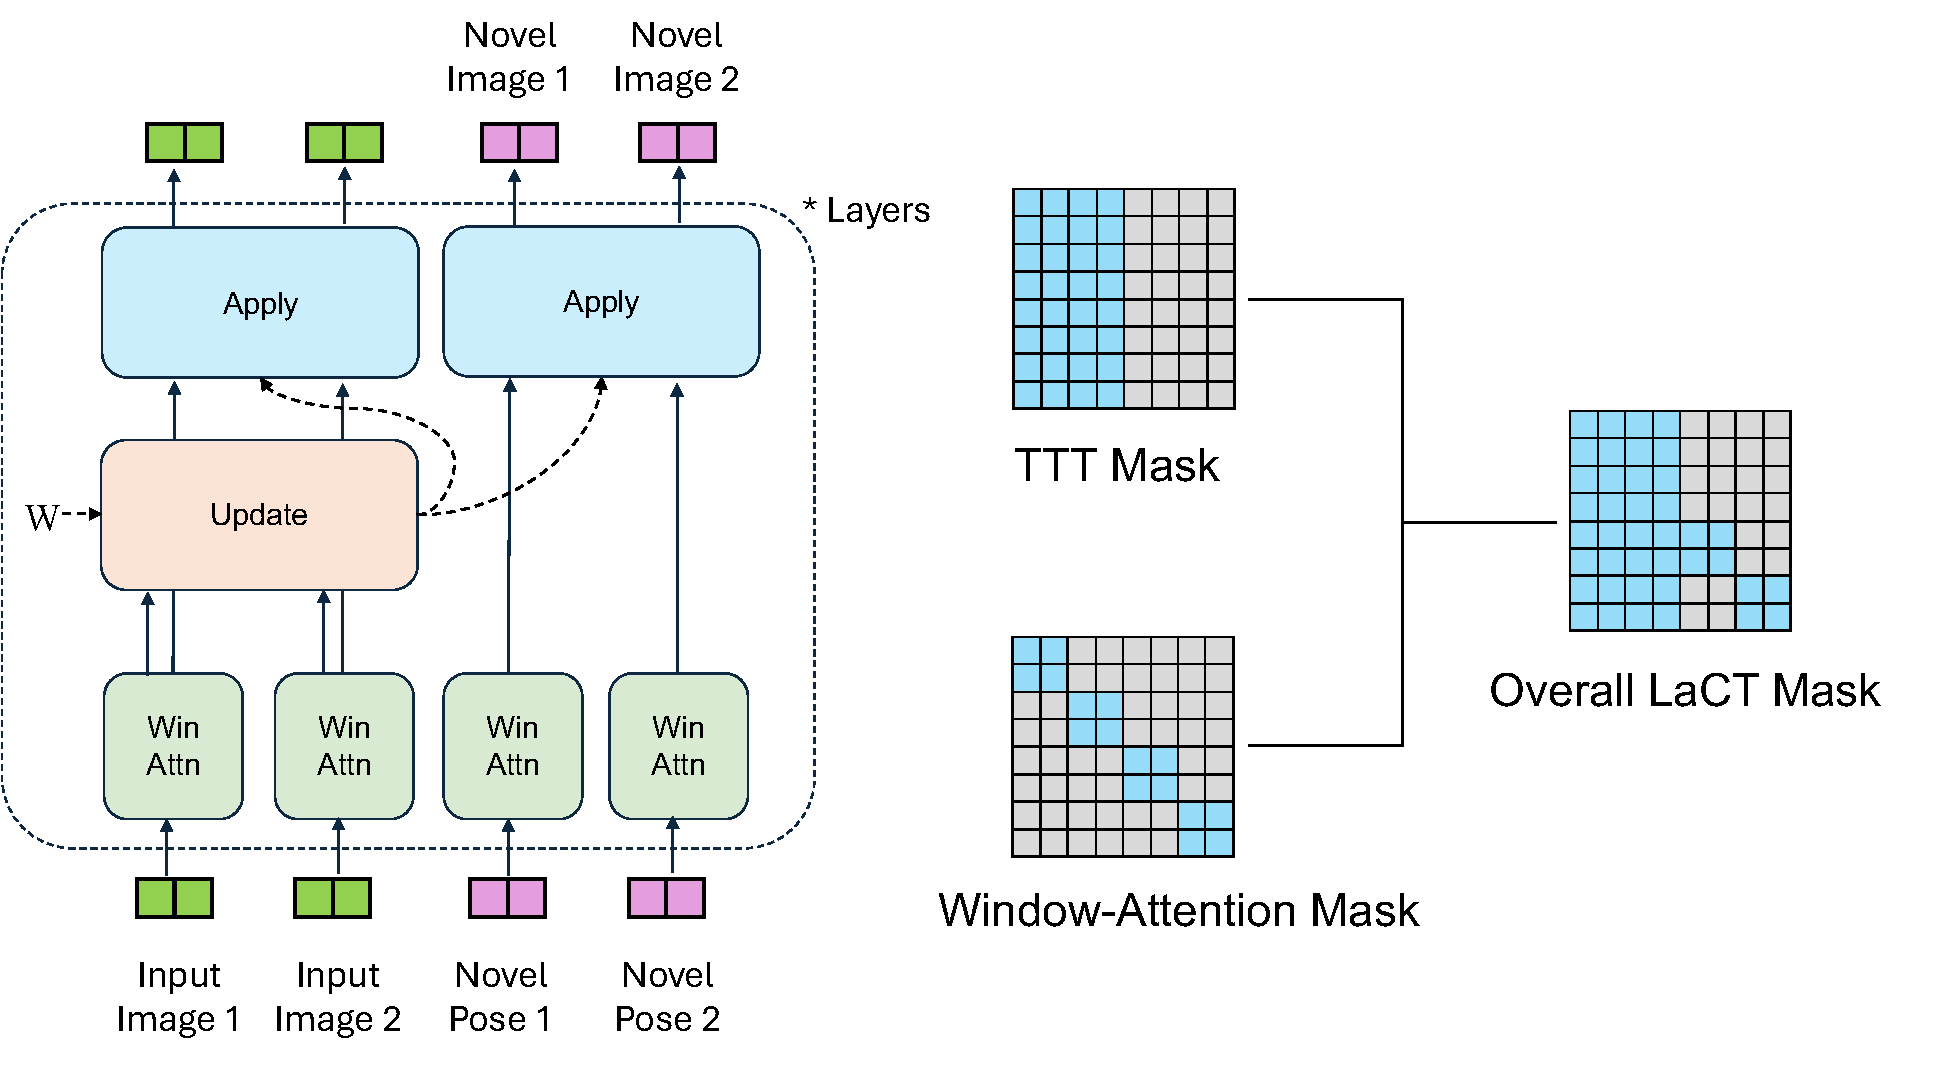
\includegraphics[width=0.8\textwidth]{figures/lvsm_model.pdf}
    % \vspace{-0.25in}
    \caption{
    Detailed \methodname{} model for our Novel-View Synthesis. Dashed line indicates flow of fast weight. Solid line indicates flow of tokens.
    Window attention is bidirectional within a single image, either the input image or the novel target image.
    TTT updates over all input tokens and apply to all tokens.
    }
    % \vspace{-0.15in}
    \label{fig:appen_lvsm_model}
\end{figure}

For actually using this model for NVS task during inference, we first get the updated fast weight with all input images.
Then, we would not change the fast weight during the rendering process (i.e., the process to convert novel camera poses to the novel images).
% The pipeline from novel camera poses to the novel image 
The \methodname{} during rendering would be similar to a ViT (Vision transformer) architecture despite having two feed-forward networks:
the feed-forward network from the fast weight stores the scene information, and the feed-forward network from the slow weight (i.e., the FFN in Fig.~\ref{fig:lact_model_arch}) stored the world knowledge like physical rendering rules.


\begin{figure}[t!]
    \centering
    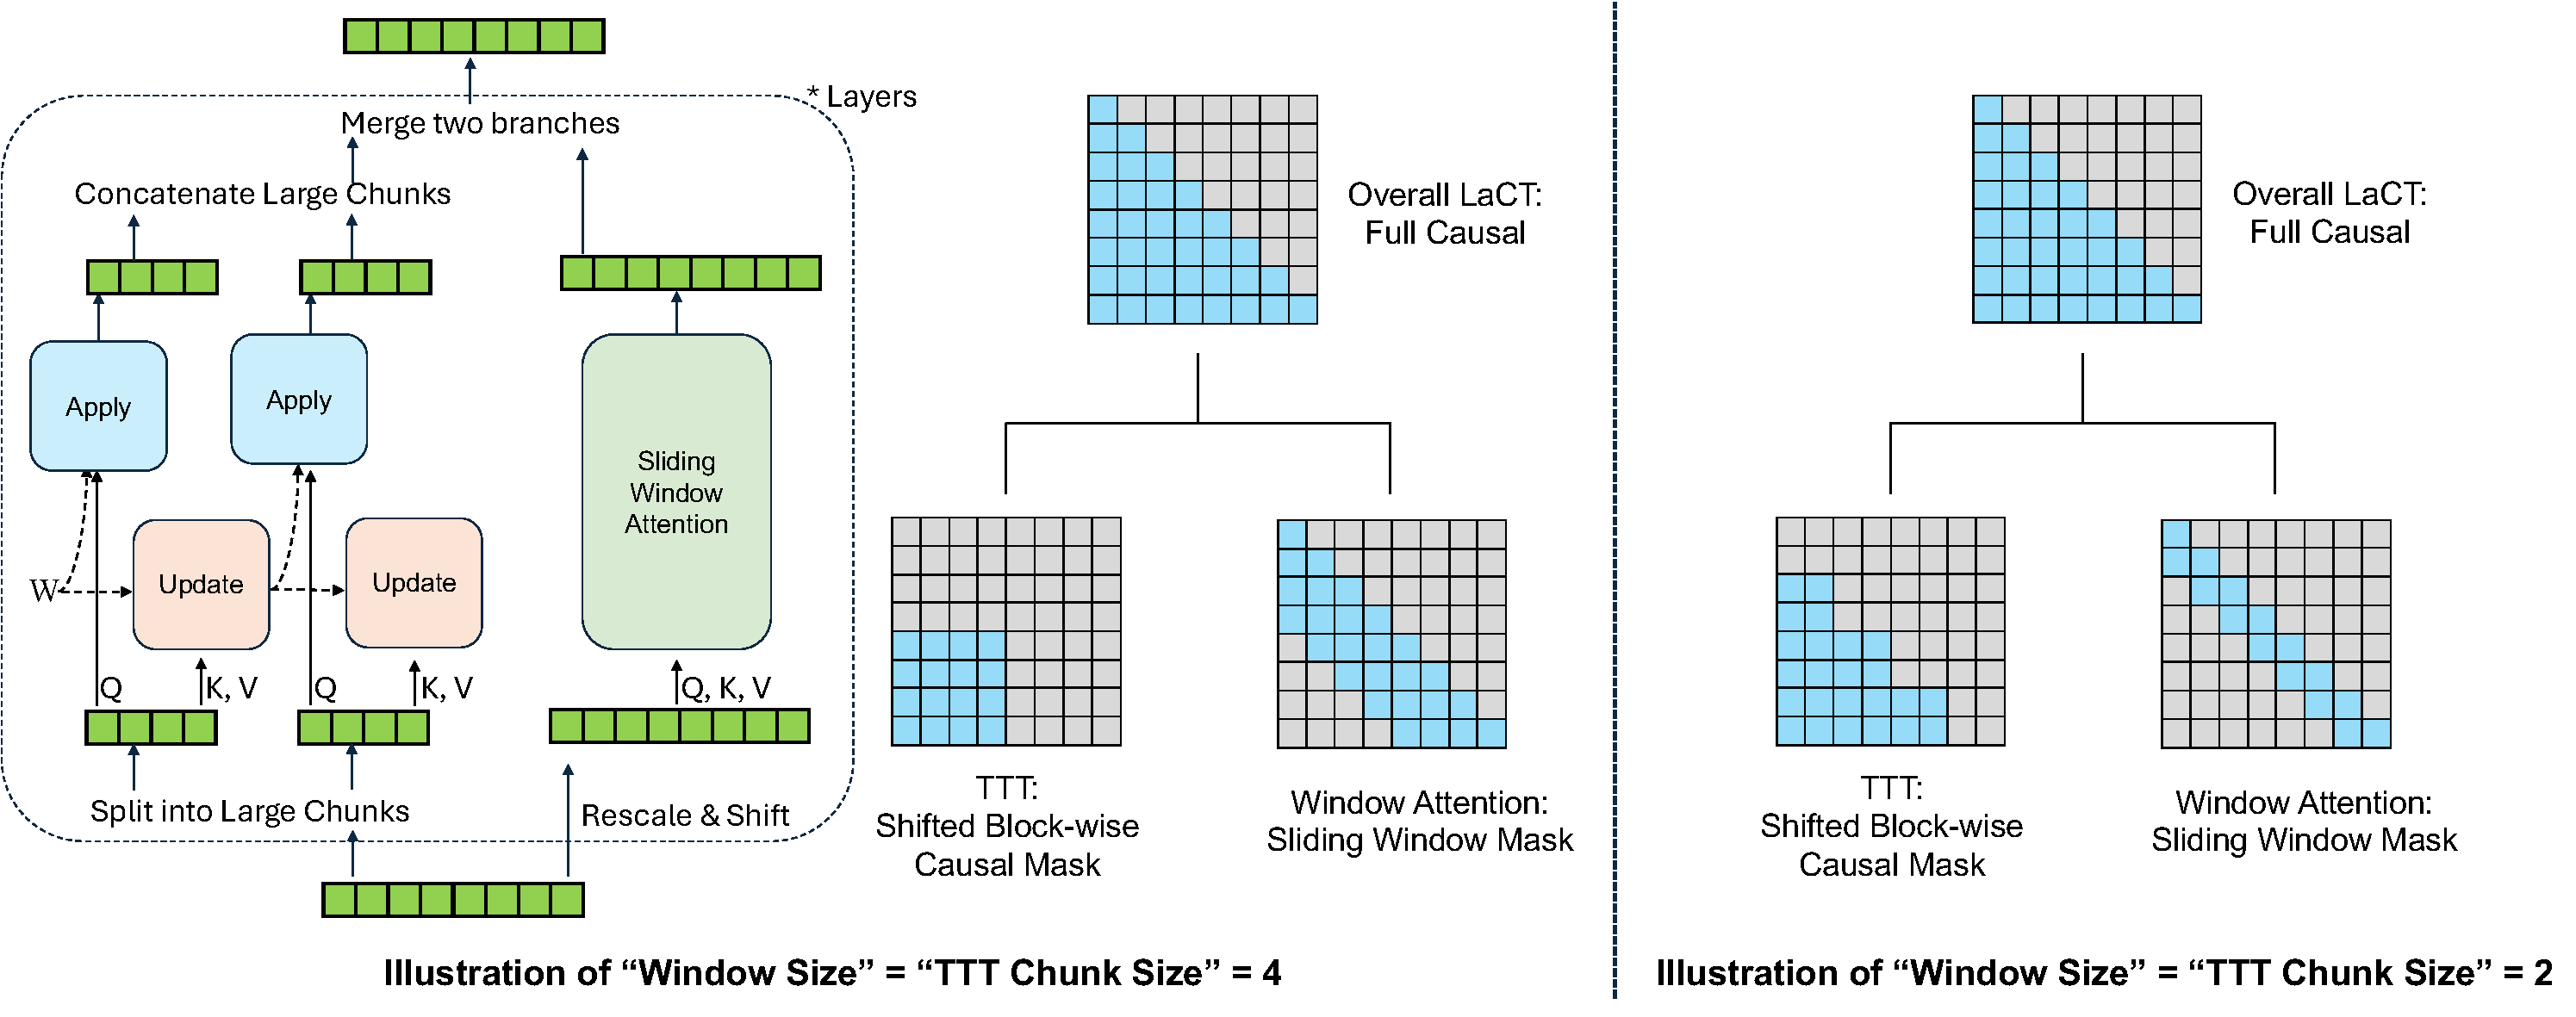
\includegraphics[width=1.0\textwidth]{figures/lm_model.pdf}
    \vspace{-0.25in}
    \caption{
    Detailed \methodname{} model for language models. Dashed line indicates flow of fast weight. Solid line indicates flow of tokens. 
    We illustrate with TTT chunk size 4 or 2, and the actual chunk size is over 2048 in \methodname{}.
    We take the parallel design for the window attention and TTT block with shared QKV.  
    The overall mask is the causal mask.
    }
    \vspace{-0.15in}
    \label{fig:appen_lm_model}
\end{figure}


\subsection{\methodname{} Architecture for Language Models}
\label{sec:appen_lm_model_arch}
Autoregressive Language Models (LM)  predicts the distribution of the next tokens $p_{\theta}(x_n|x_1, \dots, x_{n-1})$  from its history context.
It is a factorization of the full sequence distribution $p_{\theta}(x_1, \dots, x_n)$ through chain rule $p_{\theta}(x_1, \dots, x_n) = p_{\theta}(x_1)  p_{\theta}(x_2 | x_1) \ldots p_{\theta}(x_n|x_1, \dots, x_{n-1})$.
Thus it requires a token-level causal mask (demonstrated in the topright of Fig.~\ref{fig:appen_lm_model}) 
and this is the main difficulty for the large-chunk design in \methodname{}.
We use a combination of TTT layer with `Shifted Causal Block Mask' (introduced before in Fig.~\ref{fig:large_chunk_recurrence}c) and a sliding window attention to facilitate it.
By shifting the mask of TTT, it excludes the information leakage from future tokens.
As shown in the right part of Fig.~\ref{fig:appen_lm_model}, the overall dependency mask is the union of the TTT mask and the sliding window attention mask.
To achieve a token-level causal mask without bubbles, the only requirement is that the window size of the sliding window attention is greater or equal to the chunk size from the TTT.
We illustrate two example of such mask with `Window Size' = `TTT Chunk Size' = 2 or 4.
The actual chunk size and attention window size is above 2048 in our implementation for better utilization and state size scaling (discussed in Sec.~\ref{sec:efficiency_challenge}).

As illustrated in the left most of Fig.~\ref{fig:appen_lm_model}, we employ a parallel design of the TTT layer and sliding window attention to save the number of model parameters and computation FLOPs.
In details, the query (Q), key (K) and value (V) are shared between the TTT layer and window attention.
Sliding window attention is an attention with constant window size over the past history, starting from the target tokens.
For the TTT layer, we start with an apply operation over the first chunk using the initialized fast weight (i.e., unupdated yet).
The `apply' operation is followed by the `update' operation over the first chunk.
In this way, the `apply' operation would not see information inside the current chunk to avoid leaking future token information inside the chunk.
Alternatively using `apply' followed by `update' over subsequent blocks completes the desired `shifted block-wise causal mask' illustrated in Fig.~\ref{fig:appen_lm_model}.
For details of the parallel design, please refer to the Pseudocode Algorithm~\ref{alg:lact_hybrid}.

% \hao{Not sure below is correct; please verify:}
% \hao{Following GAU~\cite{hua2022transformerqualitylineartime}, the Q and Q for the TTT layer has an extra learnable scaling and shift parameters to handle the potential scaling mismatch between two layers. } \tianyuan{v does not has.  only for k and v.  only scaling and shift. ALready fixed.  when merge, learnable scalar per TTT head. }
% \hao{To merge the output of two branches, we simply add their outputs with a learnable scalar per TTT head over the TTT branch.}


We use the multi-head design for both TTT layer and window attention, although their number of heads are different.
We empirically take less number of heads for TTT layer (i.e., larger head dimension) to enable larger state size, as state size is propotional to the head dimension in our design (Sec.~\ref{sec:appen_lact_details}, and Equation~\ref{eq:state_size}). By default, we use four heads in langugae model experiments.  For positional encoding, we use the same RoPE as the window attention branch. 


\begin{figure}[t!]
    \centering
    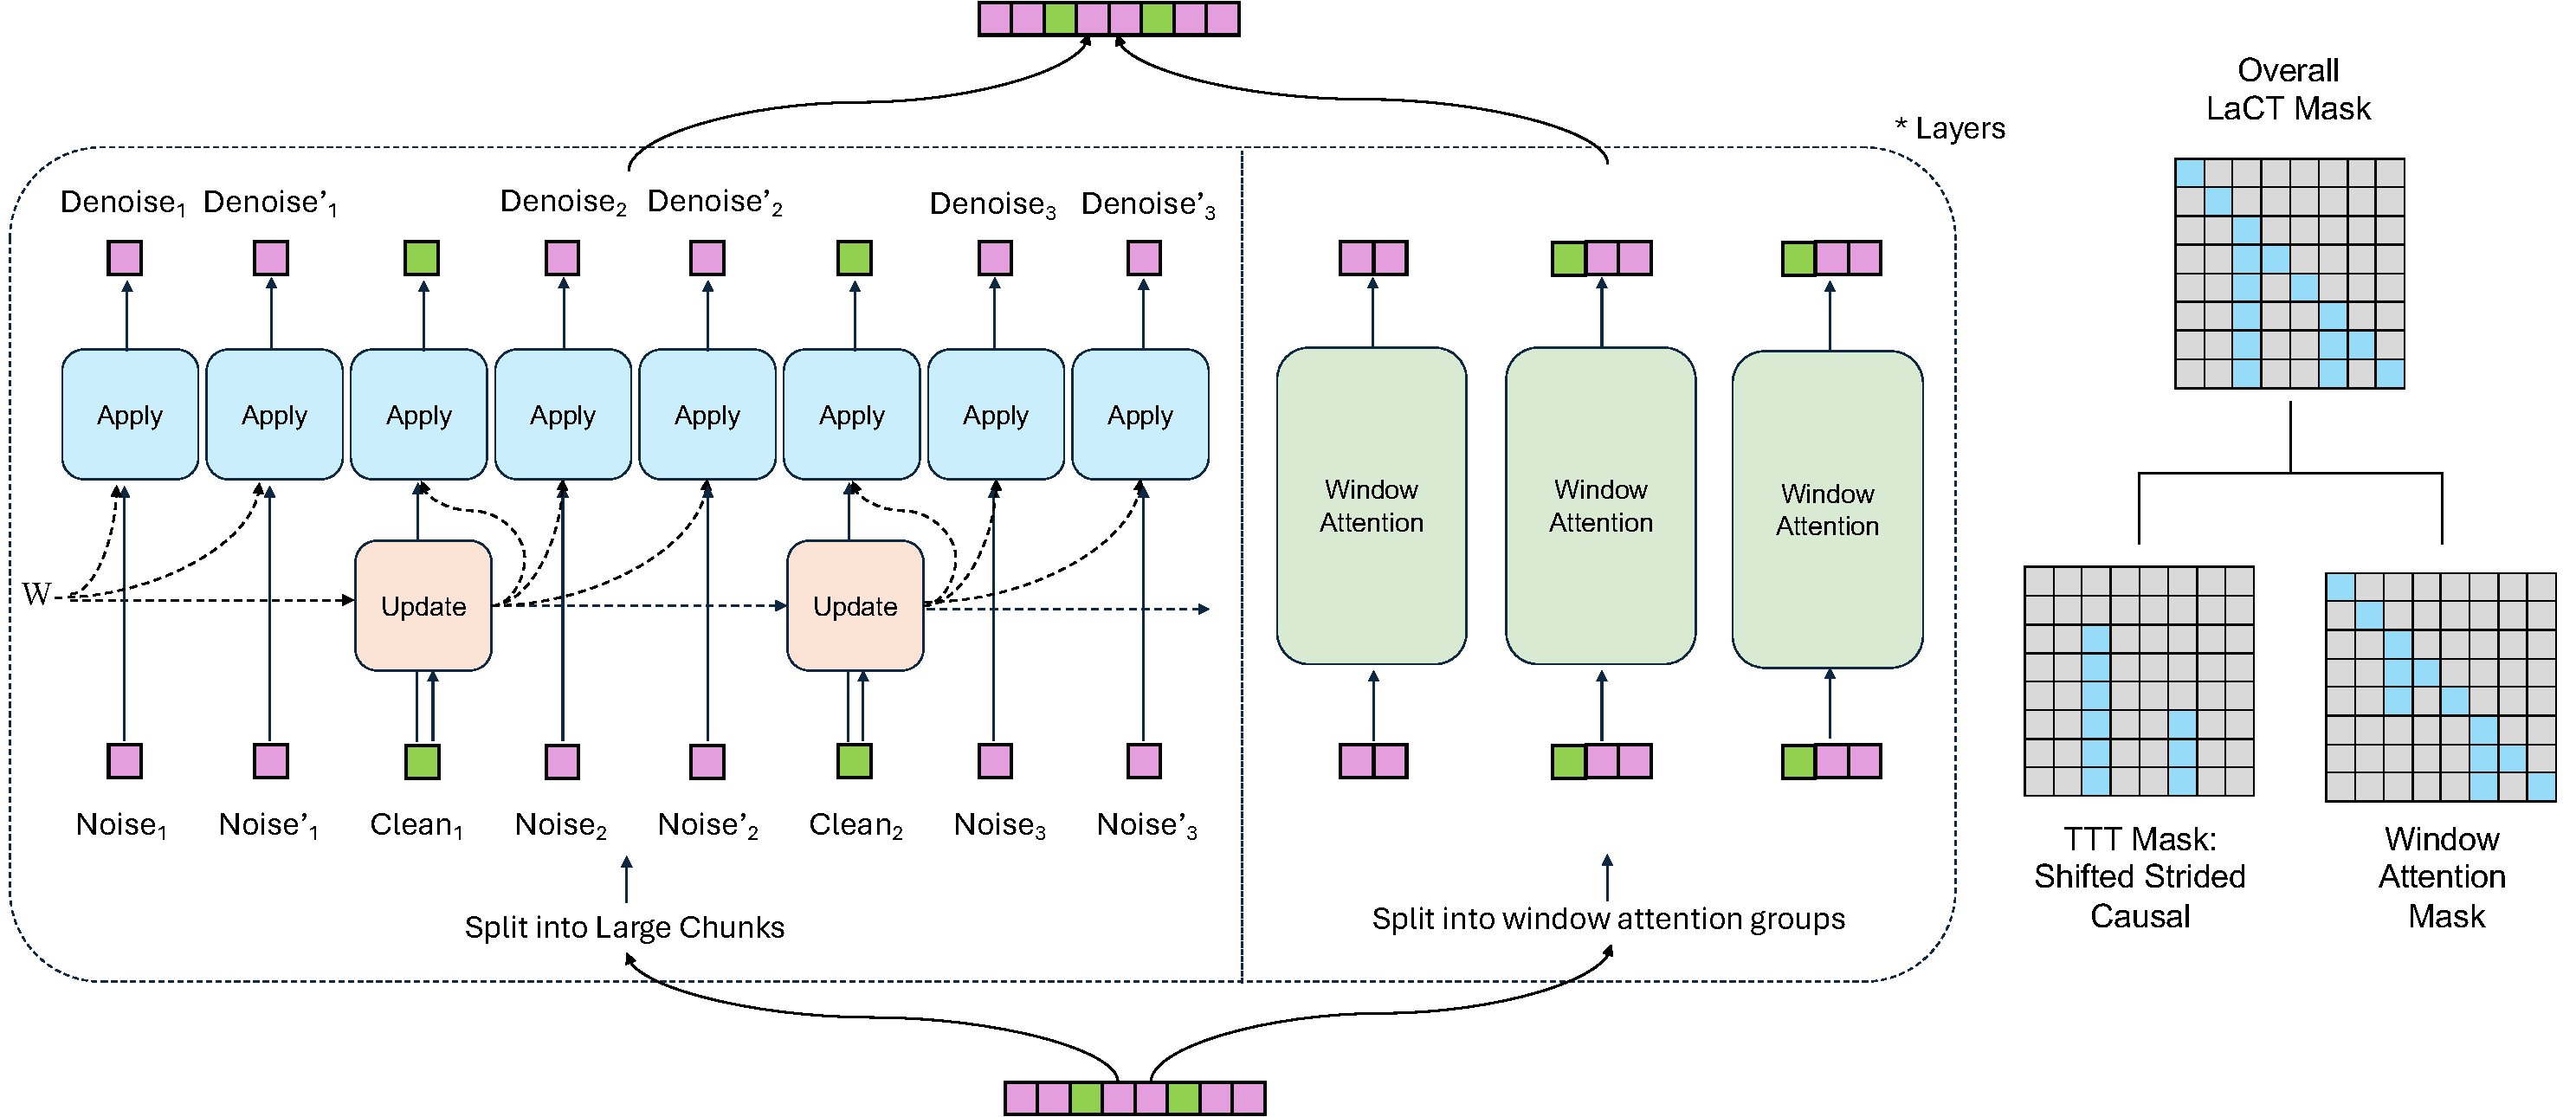
\includegraphics[width=1.0\textwidth]{figures/video_model.pdf}
    \vspace{-0.25in}
    \caption{
    Detailed \methodname{} model for autoregressive video generation by diffusion model. 
    % The tokens marked with purple color are t
    The purple tokens are noisy frame chunk for training the diffusion model.
    The green tokens are clean frame chunk.
    Each token is a large chunk in TTT, e.g., 3 consecutive frames with 4680 tokens in total.
    % We use multi-noise denoising for better utilization (detailed in Sec.~\ref{sec:exp_video}) and 
    Noise and Noise' are two noisy frames with independent Gaussian noise and time stamps over the same clean frame.
    We denoise them simultaneously to improve the utilization.
    Dashed line indicates flow of fast weight. Solid line indicates flow of tokens. 
    We take the parallel design for the window attention and TTT block with shared QKV.  
    The TTT mask is shifted  (i.e., started with apply) strided causal.
    The window attention excludes the attention from clean frame to future noisy frame, and also excludes the attention between the independent noisy frames.
    }
    \vspace{-0.15in}
    \label{fig:appen_video_model}
\end{figure}

\subsection{\methodname{} Architecture for Autoregressive Video Diffusion}
\label{sec:appen_video_model_arch}

Chunkwise autoregressive video diffusion generates videos by iteratively denoising sequential chunks of video frames, conditioned on previously generated clean frames. Each chunk can contain several video frames and span thousands of visual tokens.
We use teacher-forcing training by interleaving noisy and clean frame chunks. Specifically, a video of N frame chunks is structured as:
\begin{equation}
    S = [X_1^{\text{noise}}, X_1, X_2^{\text{noise}}, X_2, \ldots, X_N^{\text{noise}}]
    \label{eq:appen_video_sequence_basic}
\end{equation}
where each noisy chunk $X_i^{\text{noise}}$ is produced by adding unit Gaussian noise $\epsilon$ to the $i$-th clean video chunk as $X_i^{\text{noise}} = X_i (1 - t_i) + \epsilon t_i$ and $t_i \in [0, 1]$ denotes the strength of chunk-independent noise.  However, compared to previous methods that employs progressive \cite{ruhe2024rolling} or frame-independent noise strategies \cite{yin2024slow} like diffusion forcing \cite{chen2024diffusion},
our teacher-forcing formulation in Equation~\ref{eq:appen_video_sequence_basic} only uses around $50\%$ of the tokens of the entire sequence to compute the denoising loss. To improve token utilization, we consider an alternate approach by repeating each video chunk with two noise levels in the training sequence as:
\begin{equation}
    S = [X_1^{\text{noise}}, X_1^{\text{noise}_*},  X_1, X_2^{\text{noise}}, X_2^{\text{noise}_*},  X_2, \ldots, X_N^{\text{noise}}, X_N^{\text{noise}_*} ],
    \label{eq:video_sequence}
\end{equation}
where $X_i^{\text{noise}}$ and $X_i^{\text{noise}_*}$ represent two different noise levels applied to each clean video chunk $X_i$. This increases token utilization from $50\%$ to about $67\%$. While more repetition could further increase token utilization, it would also reduce training sample diversity; thus, we limit the repetition to twice. We use such repeating strategy when training the 1.3 billion parameter video diffusion model on five seconds videos. 

To process these interleaved noisy and clean chunks,  \methodname{} fast weights are updated exclusively using the clean video chunks. These updated weights are then applied to the current clean chunk and subsequent noisy chunks. The integrated local window attention uses a window size of two frame chunks and employs a block-wise causal mask. This mask allows noisy chunks to attend only to themselves and the immediately preceding clean chunk. By doing this, we main bidirectional dependies within each chunk and causal dependency across chunks. 

Similarly to our language model experiments, we integrate the TTT and local window attention into the same layer. Figure~\ref{fig:appen_video_model} illustrates this design for autoregressive video generation. The input sequence depicted in the figure follows Equation~\ref{eq:video_sequence} with each video chunk repeated twice with different noise levels. The pink color in the figure indicates noisy chunks and the green color indicates clean chunks. 




\section{Experimental Details}
\label{sec:appen_experiment_details}

\subsection{Novel View Synthesis}
\label{sec:appen_nvs_details}

\noindent\textbf{Datasets \& metric.} We evaluate our approach on 
both object-level and scene-level datasets.
We use Objaverse dataset \cite{deitke2023objaverse} for object-level training, 
and render 32 random views per object,   
following the setup from LVSM \cite{jin2024lvsm} and GS-LRM \cite{zhang2024gs}.  
% Specifically, we render 32 random views per object for 730K objects. 
After training, we perform evaluations on the Google Scanned Objects (GSO) dataset \cite{downs2022google}, at resolutions of $256\times256$ and $512\times512$.
To ensure stablized evaluation results, we render at fixed view points instead of random view points as in training.
Each evaluation involves 4–48 input views and 8 novel views per object.
For scene-level evaluations, we adopt the challenging DL3DV scene dataset~\cite{ling2024dl3dv}, which contains over 11K training scenes and 140 testing scenes, each with approximately 300 views.
% 250–300 input views and multiple novel views. 
Evaluations are performed at a resolution of $960\times536$~\footnote{The original DL3DV 960p frames released in resolution of $960\times536$. To accommodate the patch-size $8$ in our modeling, we crop it to $960\times536$ and the camera parameters are changed accordingly.  }.
We report Peak Signal-to-Noise Ratio (PSNR) in the paper's main figures, and other metrics Structural Similarity Index Measure (SSIM) and LPIPS~\cite{zhang2018unreasonable} can be found in Tables below.
For DL3DV evaluation, we follow the original paper~\cite{ling2024dl3dv} and LongLRM~\cite{ziwen2024long} to use one frame from every $8$ frame in the full video sequence as the target frames.
The input frames are from the K-means clustering of all frames as in \cite{ziwen2024long}.
% here, please refer supplementary for other metrics Structural Similarity Index Measure (SSIM) and LPIPS~\cite{zhang2018unreasonable}. 


\noindent\textbf{Model details.}
Our models consist of 24 stacked \methodname{} blocks, each with a model dimension of 768. 
The detail of such block is illustrated in Sec.~\ref{sec:appen_nvs_details}:
% every block  has a per-image window attention layer, a SwiGLU-MLP large-chunk TTT layer, and a feed-forward layer. 
Unless otherwise specified, we use a single-headed fast-weight SwiGLU-MLP with a hidden dimension of 1536. 
The window attention has 12 heads with head dimension 64, and is equipped with QK-normalization~\cite{henry2020query}.
The Feed-forward Network has 3072 as its intermediate hidden dimension.
The model has a total of 312M parameters, of which 84M are fast weights (i.e., $6 d^2$ per block).
We use an fast-weight lr initialization of $0.01$ by setting `const\_lr\_bias' in Algorithm~\ref{alg:full_lact_layer} to $\mathrm{softplus}(\text{const\_lr\_bias}) = 0.01$.
As we used Muon in fast weight update for NVS, \methodname{} is not sensitive to lr scale as discussed in Sec.~\ref{sec:update_rule}.
% }

\noindent\textbf{Baselines.}
For object-level evaluations, we compare against two baselines, including a full-attention model, 
and a register-attention model in a Perceiver style~\cite{jaegle2021perceiver}, 
In the full-attention baseline, we 
replace the TTT layer in our model with a block-wise causal attention layer, where 
the input tokens interact bidirectionally and the novel view tokens cross-attend 
to the input tokens. Such a design resembles our method's prefill and parallel 
decoding strategy described in Section~\ref{sec:method-nvs}, and the key-value caches 
of the input tokens server as scene representations for novel view renderings. 
In the Perceiver-style model, we replace half of the TTT layers with 
input-to-register full-attention layers and the remaining half with register-to-novel-view
cross-attention layers. Such a model first compresses the input tokens into a constant 
set of register tokens and then decoding the novel view tokens by attending to the registers.
For scene-level evaluations, we compare against a state-of-the-art long-sequence 3D 
reconstruction work LongLRM~\cite{ziwen2024long} that applies Mamba~\cite{gu2023mamba} hybrid with full attention to predict 
3D Gaussian splats~\cite{kerbl20233d}. 
We also include comparisons with pure optimization-based 3D Gaussian splatting methods.
Tab.~\ref{tab:attention_comparison} compares the computational complexity of the 
baseline models and our models. 

\noindent\textbf{Training details.}
For object-level experiments, we first train all the model with $671$B tokens at 8 input view and 8 novel view setting at a resolution of $256\times256$. 
We then finetune them with $512\times512$ resolution for an additional $587$B tokens. 
% \tianyuan{need hao to get the bs here}. 
% \hao{need to revise given the latest experiments}
For scene dataset, we first pre-train our model first with 32 input views and 32 novel views at $128\times128$ resolution for $1.5$T tokens, then progressively finetune at larger resolutions, larger field-of-views, and more input views.
% In the first stage of the fine-tuning, we increase the number of input views, 
The finetuning is always go with a non-squared FoV to match the raw data.
Non-squared FoV has larger view range than the squared FoV, thus is harder.
The input and novel views in fine-tuning are both 64 to support better view coverage.
% The curriculum of the fine-tuning resolution is set as $72 \times 128$, $144 \times 256$, $288 \times 512$, and $536 \times 960$.
The curriculum of the fine-tuning resolution is set as $128 \times 72$, $256 \times 144$, $512 \times 288$, and $960 \times 536$.
The training tokens for each stage is around $100$B.
High-resolution models (starting from $512 \times 288$) are trained with inner-chunk context parallelism (Sec.~\ref{sec:parallelism}). 
% See Appendix for details. 

At each training stage, we always use AdamW with linear learning rate warmup and weight decay of $0.05$.
The peak learning rate of the pre-training is $4e-4$.
During fine-tuning, we use smaller learning rate (usually $1e-5$ to $5e-5$).

The training is completed with 64 A100 GPUs.
The pre-training takes $8$ days, and each fine-tuning stage is about $12$hours (thus 2 days in total).


\noindent\textbf{Detailed Result Numbers}
We here provided the detailed number for object-level  results on the GSO dataset (at resolution $256\times256$ in Table~\ref{tab:gso_256}, $512\times512$ in Table~\ref{tab:gso_512}) and DL3DV evaluations (at resolution $960\times536$ in Table~\ref{tab:dl3dv_960p}).

% \begin{table}[h]
% \centering
% \caption{256-Res object-level novel view synthesis results on GSO. Both the input and output are with resolution $256\times256$. 
% $\uparrow$: higher is better, $\downarrow$: lower is better.}
% \resizebox{\textwidth}{!}{%
% \begin{tabular}{lccccccccc}
% \toprule
% \textbf{Input} 
% % \multirow{2}{*}{\textbf{Input Views}} 
% & \multicolumn{3}{c}{\textbf{LaCT}} 
% & \multicolumn{3}{c}{\textbf{Full Attention}} 
% & \multicolumn{3}{c}{\textbf{Perceiver Attention}} \\
% \textbf{Views} 
% & \textbf{PSNR}~($\uparrow$) & \textbf{LPIPS}~($\downarrow$) & \textbf{SSIM}~($\uparrow$) 
% & \textbf{PSNR}~($\uparrow$) & \textbf{LPIPS}~($\downarrow$) & \textbf{SSIM}~($\uparrow$) 
% & \textbf{PSNR}~($\uparrow$) & \textbf{LPIPS}~($\downarrow$) & \textbf{SSIM}~($\uparrow$) \\
% \midrule
% 4  & 32.4 & 0.030 & 0.962 & 32.6 & 0.029 & 0.964 & 30.3 & 0.039 & 0.950 \\
% 8  & 35.3 & 0.019 & 0.976 & 35.6 & 0.018 & 0.978 & 32.8 & 0.026 & 0.967 \\
% 12 & 36.3 & 0.017 & 0.980 & 36.6 & 0.015 & 0.982 & 33.6 & 0.023 & 0.971 \\
% 20 & 37.2 & 0.015 & 0.982 & 37.5 & 0.014 & 0.984 & 34.3 & 0.021 & 0.974 \\
% 32 & 37.5 & 0.014 & 0.982 & 37.9 & 0.013 & 0.985 & 34.2 & 0.021 & 0.974 \\
% 48 & 37.6 & 0.014 & 0.983 & 37.9 & 0.013 & 0.985 & 33.7 & 0.022 & 0.972 \\
% \bottomrule
% \end{tabular}
% }
% \label{tab:gso_256}
% \end{table}

\begin{table}[h]
\centering
\caption{256-Res object-level novel view synthesis results on GSO. Both the input and output are with resolution $256\times256$. 
$\uparrow$: higher is better, $\downarrow$: lower is better.}
\resizebox{\textwidth}{!}{%
\begin{tabular}{lcccccccccc}
\toprule
\textbf{Input} & \textbf{\# Input Tokens} 
& \multicolumn{3}{c}{\textbf{LaCT}} 
& \multicolumn{3}{c}{\textbf{Full Attention}} 
& \multicolumn{3}{c}{\textbf{Perceiver Attention}} \\
\textbf{Views} & 
& \textbf{PSNR}~($\uparrow$) & \textbf{LPIPS}~($\downarrow$) & \textbf{SSIM}~($\uparrow$) 
& \textbf{PSNR}~($\uparrow$) & \textbf{LPIPS}~($\downarrow$) & \textbf{SSIM}~($\uparrow$) 
& \textbf{PSNR}~($\uparrow$) & \textbf{LPIPS}~($\downarrow$) & \textbf{SSIM}~($\uparrow$) \\
\midrule
4  & 4{,}096   & 32.4 & 0.030 & 0.962 & 32.6 & 0.029 & 0.964 & 30.3 & 0.039 & 0.950 \\
8  & 8{,}192   & 35.3 & 0.019 & 0.976 & 35.6 & 0.018 & 0.978 & 32.8 & 0.026 & 0.967 \\
12 & 12{,}288  & 36.3 & 0.017 & 0.980 & 36.6 & 0.015 & 0.982 & 33.6 & 0.023 & 0.971 \\
20 & 20{,}480  & 37.2 & 0.015 & 0.982 & 37.5 & 0.014 & 0.984 & 34.3 & 0.021 & 0.974 \\
32 & 32{,}768  & 37.5 & 0.014 & 0.982 & 37.9 & 0.013 & 0.985 & 34.2 & 0.021 & 0.974 \\
48 & 49{,}152  & 37.6 & 0.014 & 0.983 & 37.9 & 0.013 & 0.985 & 33.7 & 0.022 & 0.972 \\
\bottomrule
\end{tabular}
}
\label{tab:gso_256}
\end{table}


\begin{table}[h]
\centering
\caption{512-Res object-level novel view synthesis results on GSO. Both the input and output are with resolution $512\times512$ comparison across methods. $\uparrow$: higher is better, $\downarrow$: lower is better.}
\resizebox{0.85\textwidth}{!}{%
\begin{tabular}{lccccccc}
\toprule
\multirow{2}{*}{\textbf{Input Views}}
& \multirow{2}{*}{\textbf{\# Input Tokens}}
& \multicolumn{3}{c}{\textbf{LaCT}} 
& \multicolumn{3}{c}{\textbf{Full Attention}} \\
& 
& \textbf{PSNR}~($\uparrow$) & \textbf{LPIPS}~($\downarrow$) & \textbf{SSIM}~($\uparrow$) 
& \textbf{PSNR}~($\uparrow$) & \textbf{LPIPS}~($\downarrow$) & \textbf{SSIM}~($\uparrow$) \\
\midrule
4   & 16{,}384   & 33.4 & 0.029 & 0.969 & 33.6 & 0.027 & 0.971 \\
8   & 32{,}768   & 36.6 & 0.020 & 0.979 & 36.7 & 0.017 & 0.982 \\
12  & 49{,}152   & 37.7 & 0.017 & 0.983 & 37.9 & 0.015 & 0.985 \\
20  & 81{,}920   & 38.6 & 0.016 & 0.984 & 38.9 & 0.013 & 0.987 \\
32  & 131{,}072  & 39.0 & 0.015 & 0.985 & 39.3 & 0.013 & 0.988 \\
48  & 196{,}608  & 39.1 & 0.015 & 0.985 & 39.3 & 0.012 & 0.988 \\
\bottomrule
\end{tabular}
}
\label{tab:gso_512}
\end{table}



\begin{table}[h]
\centering
\caption{960P scene-level novel view synthesis results for LaCT on DL3DV. Both the input and output are with resolution $960\times536$ (width x height). $\uparrow$: higher is better, $\downarrow$: lower is better.}
\resizebox{0.55\textwidth}{!}{%
\begin{tabular}{lcccc}
\toprule
\textbf{Input Views} 
& \textbf{\# Input Tokens} 
& \textbf{PSNR}~($\uparrow$) 
& \textbf{LPIPS}~($\downarrow$) 
& \textbf{SSIM}~($\uparrow$) \\
\midrule
16  & 128{,}640  & 24.7 & 0.224 & 0.793 \\
32  & 257{,}280  & 26.9 & 0.185 & 0.837 \\
64  & 515{,}520  & 28.3 & 0.169 & 0.857 \\
128 & 1{,}031{,}520 & 28.9 & 0.166 & 0.861 \\
\bottomrule
\end{tabular}
}
\label{tab:dl3dv_960p}
\end{table}




% \hao{For numbers not included in the above tables, feel free to reach out to authors.}


\subsection{Language Modeling}\label{sec:appen_exp_language}


\noindent\textbf{Datasets \& Metrics.}
We train our models on the Long-Data-Collections dataset~\cite{long_data_collection}, containing approximately 68.8B tokens tokenized using Mixstra tokenizer (32,000 codebook size).
The dataset is a mix of 41.4\% General Data (e.g., RedPajama-Book, RedPajama-ArXiv, 1B tokens from RedPajama, and a Pile subsample) and 58.6\% Instruction Data (e.g., UL2 Oscar, NI, and P3). 
To evaluate long-context capabilities, we utilized the per-token loss metric from~\cite{linforgetting}. A consistently decreasing per-token loss across the input sequence indicates effective use of the entire context, while a plateau suggests an inability to leverage information beyond that point. Specifically, we evaluated next-token prediction loss on 2.5B tokens from the Book-3 dataset~\cite{gao2020pile} for our 760M-parameter model, and on 5B tokens for our 3B-parameter model. Additionally, we measured retrieval accuracy using the RULER benchmark~\cite{hsiehruler} across various sequence lengths to assess context memorization and information retrieval, evaluating up to the trained sequence length.

\noindent\textbf{Model details.}
We modified the original \methodname{} block by removing its window-attention layer. Instead, we incorporate a causal sliding window-attention(SWA) layer directly into the Large-Chunk TTT layer. The SWA layer shares the same Q, K, and V vectors
as the fast-weight network, except that a per-channel leranable scale and shift is applied  
to Q and K before they are fed to the SWA layer (as done in GAU~\cite{hua2022transformer}).  We sum up the output of the SWA layer and that of the TTT layer, where the output of the TTT layer is scaled by 
another per-head learnable scalar. 
We use an fast-weight lr initialization of $0.001$ by setting `const\_lr\_bias' in Algorithm~\ref{alg:full_lact_layer} to $\mathrm{softplus}(\text{const\_lr\_bias}) = 0.001$.
% }
We illustrate this archtecture in Figure~\ref{fig:appen_lm_model}. 

To ensure a fair comparison with baselines in terms of trainable parameters.we adjusted the \methodname{} block's extra learnable initial fast weights $W = [W_1, W_2, W_3]$. o reduce parameters, we employed a low-rank version for $W_1, W3$ with a rank of 32. For instance, if $W_1 \in \mathcal{R}^{d\times d}$, its low-rank initial fast weight is $W_1 = L \cdot R + 0.5 * I_d$, where $L \in \mathcal{R}^{d\times32}, R \in \mathcal{R}^{32\times d}$, and $I_d$ is identity matrix. This reduces the extra trainable parameters for the fast weights in each block to $128 * \text{model-dim} + \frac{1}{\text{num-heads}} (\text{model-dim}^2) $. Additional minor parameters for learning rate projection, per-head scalers, an extra RMSNorm, and the SWA's learnable scale and shift are of order $O(\text{model-dim})$.  Standard blocks typically have $12 \cdot \text{model-dim}^2$ parameters. Our approach adds approximately $\frac{1}{\text{num-heads}} (\text{model-dim}^2)$ extra parameters, which is less than 3\% of total trainable weights with four heads, and below 4.5\% with two heads.  By default, \methodname{} use four heads in the experiments, unless noted otherwise, which means that the default state size per block is $\frac{3}{4} (\text{model-dim}^2)$. 


\noindent\textbf{Baselines.}
We compare our approach with full attention, Gated Linear Attention (GLA)~\cite{yang2024gated}, DeltaNet~\cite{schlag2021linear,yangparallelizing}. To ensure fairness, we enhance both GLA and DeltaNet with the same sliding window attention.  As pointed out in previous work \cite{linforgetting, xiong2023effective, men2024base}, a large RoPE~\cite{su2023roformer} base is critical for transformers in long-context training, thus we adopt a large RoPE base of 1 million for training with 32K token contexts whenever softmax attention is used.
Tab.~\ref{tab:appen_LM_baseline} compares the mechanism and computing complexity of the baseline methods and our method. Training throughput (tokens per second per GPU, TPS) was using a 3B-parameter model on eight A100-40GB SXM4 GPUs with activation checkpointing and FSDP. At the 3 billion parameter scale, all models use 24 softmax attention heads.  The GLA baseline has eight linear attention heads with heads dimension as 384, resulting in a total state size of $384d$, with $d=3072$ representing the model dimension.  DeltaNet employs 24 linear attention heads, each with a dimension of 128, leading to a total state size of $128d$. Our approach uses four TTT heads with head dimension as $768$, and since each block has three fast weights, the total state size is $2304d$. 



\begin{table*}[htbp]
\centering
\caption{Comparison of baseline methods in terms of state size, training throughput (measured in tokens per second, TPS), update rules, and memory read-out mechanisms. Training throughput is evaluated using a 3B-parameter model with 32K-sequence length on A100-40GB GPUs.}
\label{tab:appen_LM_baseline}
\resizebox{\textwidth}{!}{%
\begin{tabular}{llllll}
\toprule
 & \textbf{State size}  & \textbf{Train TPS} &  \textbf{Update Rule} & \textbf{Memory read-out} \\
\midrule
Transformer     & –       & 4.1K     & – & – \\
Transformer SWA & –       & 6.4K   & – & – \\
\midrule
\multicolumn{5}{l}{ \textit{Per-token recurrence} } \\
GLA SWA         & $384d$  & 5.0K   &
$\displaystyle \mathbf{S}_t \leftarrow  \mathbf{S}_{t-1}\mathrm{Diag}(\boldsymbol{\alpha}_t) + \mathbf{v}_t \mathbf{k}_t^\top$ 
& $\displaystyle \mathbf{o}_t = \mathbf{S}_t \mathbf{q}_t$ \\
DeltaNet SWA    & $128d$  & 5.1K   &
$\displaystyle \mathbf{S}_t \leftarrow  \mathbf{S}_{t-1}(\mathbf{I} - \beta_t \mathbf{k}_t \mathbf{k}_t^\top) + \beta_t \mathbf{v}_t \mathbf{k}_t^\top$ 
& $\displaystyle \mathbf{o}_t = \mathbf{S}_t \mathbf{q}_t$ \\
\midrule
\multicolumn{5}{l}{ \textit{Large-chunk recurrence} } \\
Ours GD       & $2304d$ & 5.0K    
& $ W \leftarrow \mathrm{L2norm}(W - \sum_i^b \eta_i \nabla_W \mathcal{L}_i)$
& $\displaystyle \mathbf{o}_t = f_W(\mathbf{q}_t)$  \\
Ours  Momentum       & $2304d$ & 4.9K    
& $M \leftarrow \beta M + \sum_i^b \eta_i \nabla_W \mathcal{L}_i;\; W \leftarrow  \mathrm{L2norm}(W - M)$
& $\displaystyle \mathbf{o}_t = f_W(\mathbf{q}_t)$  \\
Ours Muon       & $2304d$ & 4.3K  
& $ M \leftarrow  \beta M + \sum_i^b \eta_i \nabla_W \mathcal{L}_i;\;  W \leftarrow  \mathrm{L2norm}(W - \mathrm{Muon}(M))$
& $\displaystyle \mathbf{o}_t = f_W(\mathbf{q}_t)$ \\
\bottomrule
\end{tabular}%
}
\end{table*}

\noindent\textbf{Training Details.}
We trained models at two scales using a sequence length of 32,768 tokens:

\begin{itemize}
    \item 760M parameters: We use 24 stack blocks, with model dimension as $1536$. All models are trained for 40B tokens (40,960 steps) with a sliding window of 2048 tokens and a batch size of 1 million tokens. Each experiment ran on 32 A100-40GB SXM GPUs for approximately 20 hours.
    \item 3B parameters: We use 25 stack blocks, with model dimension as $3072$. All models are trained for 60B tokens (30,000 steps) with a sliding window of 4096 tokens and a batch size of 2 million tokens. Each experiment ran on 64 A100-40GB SXM GPUs for approximately 50-60 hours.
\end{itemize}
For both scales, we used a base learning rate of $1\times 10^{-3}$ 
 with a cosine decay scheduler and 1024 warmup steps. All models were randomly initialized with a standard deviation of 0.02.

\noindent\textbf{Results.} Detailed results on the RULER benchmark~\cite{hsiehruler} are presented in Tables~\ref{tab:ruler-single} and ~\ref{tab:ruler-multi}. We evaluated models on S-NIAH-1, S-NIAH-2, and S-NIAH-3 tasks, which represent varying difficulties of the single "needle in a haystack" retrieval. We also report performance on NIAH-MultiKey-1, NIAH-MultiQuery, and NIAH-MultiValue. Other RULER tasks are not reported as the full attention baseline also achieved trivial results beyond a 16K sequence length.


\begin{table}[ht]
\centering
\caption{RULER benchmark results for Single Needle in a Haystack (S-NIAH) tasks. * Our method with two heads (default is four).}
\label{tab:ruler-single}
\resizebox{\textwidth}{!}{%
\begin{tabular}{lcccc|cccc|cccc|cccc}
\toprule
& \multicolumn{4}{c}{S-NIAH-1} & \multicolumn{4}{c}{S-NIAH-2} & \multicolumn{4}{c}{S-NIAH-3} & \multicolumn{4}{c}{Average} \\
\cmidrule(lr){2-5}\cmidrule(lr){6-9}\cmidrule(lr){10-13}\cmidrule(lr){14-17}
Model & 4K & 8K & 16K & 32K & 4K & 8K & 16K & 32K & 4K & 8K & 16K & 32K & 4K & 8K & 16K & 32K \\
\midrule
\multicolumn{17}{l}{\textit{760M parameters}} \\
Transformer & 99.2 & 96.6 & 85.2 & 68.0 & 100 & 100 & 85.8 & 82.2 & 81.0 & 73.8 & 74.8 & 36.8 & 93.4 & 90.1 & 81.9 & 62.3 \\
DeltaNet + SWA & 84.0 & 85.2 & 87.8 & 86.8 & 62.8 & 29.4 & 14.2 & 7.8 & 53.8 & 21.8 & 11.2 & 5.8 & 66.9 & 45.5 & 37.7 & 33.5 \\
GLA + SWA & 51.8 & 26.2 & 14.4 & 8.6 & 55.8 & 26.4 & 15.8 & 7.8 & 58.0 & 23.8 & 16.2 & 5.0 & 55.2 & 25.5 & 15.5 & 7.1 \\
Ours & 94.8 & 53.2 & 26.0 & 14.8 & 74.0 & 28.0 & 14.2 & 7.8 & 42.8 & 26.6 & 14.4 & 6.8 & 70.5 & 35.9 & 18.2 & 9.8 \\
Ours Momentum & 95.6 & 84.8 & 83.4 & 84.8 & 91.4 & 73.4 & 22.8 & 7.8 & 82.6 & 34.8 & 16.6 & 6.6 & 89.9 & 64.3 & 40.9 & 33.1 \\
Ours Momentum* & 59.0 & 30.0 & 12.4 & 8.4 & 93.4 & 50.0 & 18.2 & 7.8 & 60.2 & 25.6 & 14.2 & 6.8 & 70.9 & 35.2 & 14.9 & 7.7 \\
Ours Muon & 98.0 & 95.0 & 92.2 & 92.4 & 86.6 & 60.2 & 17.0 & 7.8 & 49.2 & 26.2 & 10.9 & 5.2 & 77.9 & 60.5 & 40.0 & 35.1 \\
\midrule
\multicolumn{17}{l}{\textit{3B parameters}} \\
Transformer & 100 & 100 & 100 & 100 & 100 & 99.8 & 100 & 98.6 & 98.6 & 95.8 & 90.8 & 75.0 & 99.5 & 98.5 & 96.9 & 91.2 \\
GLA SWA & 100 & 52.8 & 26.0 & 13.2 & 100 & 51.8 & 29.6 & 14.4 & 98.0 & 54.4 & 27.6 & 12.4 & 99.3 & 53.0 & 27.7 & 13.3 \\
DeltaNet SWA & 100 & 89.6 & 76.2 & 54.8 & 100 & 76.4 & 42.2 & 17.0 & 90.6 & 57.6 & 27.4 & 13.4 & 96.9 & 74.5 & 48.6 & 28.4 \\
Ours Momentum & 99.4 & 97.0 & 98.6 & 93.4 & 100 & 75.6 & 39.6 & 15.0 & 91.8 & 63.0 & 27.8 & 13.4 & 97.1 & 78.5 & 55.3 & 40.6 \\
Ours Muon & 98.8 & 99.2 & 98.6 & 93.4 & 100 & 99.0 & 83.2 & 30.8 & 95.4 & 90.8 & 55.6 & 19.8 & 98.1 & 96.3 & 79.1 & 48.0 \\
\bottomrule
\end{tabular}%
}
\end{table}




\begin{table}[ht]
\centering
\caption{Performance on Multi-Key (MK-NIAH), Multi-Query (MQ-NIAH), and Multi-Value (MV-NIAH) Needle in a Haystack tasks from the RULER benchmark. * Our method with two heads (default is four).}
\label{tab:ruler-multi}
\resizebox{\textwidth}{!}{%
\begin{tabular}{lcccc|cccc|cccc|cccc}
\toprule
 & \multicolumn{4}{c}{MK-NIAH} 
 & \multicolumn{4}{c}{MQ-NIAH} 
 & \multicolumn{4}{c}{MV-NIAH} 
 & \multicolumn{4}{c}{Average} \\
\cmidrule(lr){2-5}\cmidrule(lr){6-9}\cmidrule(lr){10-13}\cmidrule(lr){14-17}
Model 
 & 4K & 8K & 16K & 32K 
 & 4K & 8K & 16K & 32K 
 & 4K & 8K & 16K & 32K 
 & 4K & 8K & 16K & 32K \\
\midrule
\multicolumn{17}{l}{\textit{760M parameters}} \\
Transformer
 & 63.8 & 72   & 71.4 & 54    
 & 33.4 & 28.9 & 24   & 23.1  
 & 27.95 & 24   & 20.5 & 27.35
 & 41.7 & 41.6 & 38.6 & 34.8 \\
DeltaNet+SWA 
 & 41.2 & 30 & 14.6 & 8.2    
 & 33   & 22.45 & 7.5 & 4.3    
 & 32.4 & 22.8 & 9.15 & 6.6
 & 35.5 & 25.1 & 10.4 & 6.4 \\
GLA + SWA 
 & 45.4 & 28.4 & 15.8 & 6.6
 & 26.1 & 17.75 & 10.2 & 5.85
 & 25.4 & 16.85 & 10.1 & 6.6
 & 32.3 & 21.0 & 12.0 & 6.3 \\
Ours 
 & 60.8 & 34.6 & 16.8 & 7
 & 35   & 23.65 & 14.1 & 7.45
 & 20.7 & 22.05 & 12.7 & 6.85
 & 38.8 & 26.8 & 14.5 & 7.1 \\
Ours Momentum 
 & 62 & 41 & 21.2 & 10.4 
 & 35.3 & 24.95 & 17.7 & 8.6 
 & 27.9 & 23.15 & 16.65 & 8.2
 & 41.7 & 29.7 & 18.5 & 9.1 \\
Ours Momentum* 
 & 59.8 & 37.8 & 19.2 & 8.8
 & 36.65 & 20.45 & 12.5 & 7.4
 & 24.45 & 16.95 & 11.6 & 6.8
 & 40.3 & 25.1 & 14.4 & 7.7 \\
Ours Muon 
 & 62.8 & 46.6 & 22 & 8.6 
 & 37.7 & 26.55 & 15.7 & 7.1
 & 28.35 & 23.15 & 13.6 & 6.85
 & 42.9 & 32.1 & 17.1 & 7.5 \\
\midrule
\multicolumn{17}{l}{\textit{3B parameters}} \\
Transformer 
 & 95 & 90.4 & 81.6 & 65.2
 & 86.45 & 81.55 & 71.70 & 40.85
 & 61.8 & 42.8 & 30.75 & 22.9
 & 81.1 & 71.6 & 61.4 & 43.0 \\
GLA 3B  
 & 78 & 45.8 & 28.6 & 14.4
 & 50.05 & 28.05 & 19 & 10.7
 & 29.4 & 21.4 & 16.75 & 9.9
 & 52.5 & 31.8 & 21.4 & 11.7 \\
DeltaNet SWA 
 & 75.8 & 57.4 & 34.2 & 17.8
 & 66.25 & 33.05 & 21.45 & 13.45
 & 43.7 & 23.2 & 18.85 & 13.2
 & 61.9 & 37.9 & 24.8 & 14.8 \\
Ours Momentum 
 & 96.2 & 59.6 & 35 & 17.2 
 & 87.05 & 40.25 & 25.6 & 13.2  
 & 88.08 & 30.65 & 21.9 & 12.3 
 & 90.4 & 43.5 & 27.5 & 14.2 \\
Ours Muon 
 & 75.2 & 69.2 & 46.2 & 25.2
 & 44.75 & 39.1 & 24.9 & 19
 & 26.55 & 29.1 & 25.05 & 19.3
 & 48.8 & 45.8 & 32.0 & 21.2 \\
\bottomrule
\end{tabular}%
}
\end{table}



\subsection{Autoregressive Video Diffusion}
\label{sec:appen_exp_video}
We fine-tune the pretrained Wan 2.1~\cite{wang2025wan} text-to-video diffusion model into an autoregressive video diffusion model, that generates videos by iteratively denoising successive chunks of video frames.

% Specifically, we replace all bidirectional attention layers with our \methodname{} layers combined with sliding window attention. The sliding window attention uses a window size spanning two autoregressive chunks. Figure~\ref{fig:appen_video_model} illustrate the detailed architecture. 


\noindent\textbf{Model details.}  The original Wan 2.1 is a bidirectional diffusion transformer operating on the latent space of a causal video VAE, which performs 8x spatial and 4x temporal downsampling. The diffusion transformer uses a $2\times2\times1$ patchification layer to convert VAE video latents to tokens.   Each block of the diffusion transformer comprises an MLP layer, a bidirectional self-attention layer for visual tokens, and a cross-attention layer for visual and text tokens. 



Our primary modification is to the bidirectional self-attention. We first replace it with block-causal sliding window attention (SWA), using a window size of two chunks of video frames. We then integrate our \methodname{} into the same layer. We initialize learnable fast weights for \methodname{}. Consistent with our language modeling experiments, SWA and our test-time training mechanism are combined within each layer: Q and K vectors are rescaled and shifted before input to the test-time training operation. The outputs of SWA and the test-time training layer are summed, with a per-head learnable scalar (from a zero-initialized linear projection) applied to the latter. We do not use Muon in the fast-weight update, as it showed no significant difference in validation loss empirically. 
We use an fast-weight lr initialization of $0.001$ by setting `const\_lr\_bias' in Algorithm~\ref{alg:full_lact_layer} to $\mathrm{softplus}(\text{const\_lr\_bias}) = 0.001$.
This allows small update to the fast weight in the beginning of the fine-tuning.  To maintain minimal changes to the original Wan architecture, \methodname{} layers utilize the original RoPE from the Wan model, and we remove the SiLU activation function previously applied to queries and values.
 
% During teacher-forcing training, the input sequence consists of interleaved noisy and clean chunks (Equation~\ref{eq:video_sequence_basic}), where each chunk comprises three latent frames (4680 tokens). To maintain block-wise causal dependency, fast weights are updated only using clean chunks and subsequently applied to tokens of the current clean chunk and the following noisy chunks. Figure~\ref{fig:appen_video_model} details this architecture.

\noindent\textbf{Datasets.} We fine-tune the model using an internal, filtered proprietary collection of videos, each accompanied by a short text prompt generated by a visual language model\cite{chen2024internvl}.

\noindent\textbf{Training details.}
Following~\cite{esser2403scaling, wang2025wan}, we use time-step shifting (scale factor 3.0) and logit-normal denoising loss weighting (mean=0.5, std=1.0). We also apply an exponential moving average with a decay rate of 0.995 to the model weights.  Each 5-second video (16 FPS, 480×832 resolution) is encoded by the Wan VAE into a [21,60,104] latent representation. Denoising is performed autoregressively in chunks of three latent frames (4680 visual tokens each). We employ teacher-forcing with an interleaved noisy-clean chunk sequence (see Section~\ref{sec:method-arvideo}). 

\begin{itemize}
    \item \textbf{1.3B Parameter Model:} For initial training on 5-second videos, noisy chunks are repeated twice. This results in sequences of 60 latent frames (14 noisy, 6 clean chunks), totaling 93,600 tokens. We finetune the model with a batch size of 64 for 5000 iterations. The base learning rate is set to $2\times10^{-5}$ with a linear warm-up of 1000 iterations and linear decay.  Subsequently, the model is fine-tuned on 10-second video clips for 1,000 iterations. These clips correspond to 42 latent frames for the clean video portion, forming an interleaved sequence of 81 latent frames (approximately 126K tokens including noisy chunks).   Training for 5-second videos takes $\sim$20 seconds per iteration on 64 A100 80GB SXM GPUs (or $\sim$10 seconds on 64 H100 80GB SXM GPUs).
    \item  \textbf{14B Parameter Model:}. To manage GPU memory usage, noisy chunks are not repeated in this setting. We train the model on five-second videos with a batch size of 64 for 5000 iterations with a base learning rate of $5\times10^{-6}$, and use a sequence parallel size of 2 GPUs. This phase takes $\sim$80 seconds per iteration on 64 A100 GPUs. The model is then fine-tuned on 8.8-second video clips (36 latent frames for the clean portion) for an additional 600 iterations, using sequence parallelism (4 GPUs). This fine-tuning takes $\sim$80 seconds per iteration on 64 H100 GPUs.
\end{itemize}


\noindent\textbf{Baselines.}
We compare our method with three baselines: sliding window attention, Mamba2~\cite{dao2024transformers} with sliding window attention, and full block-wise causal attention, where the window attention in the baselines is implemented the same as in our model. 
For the Mamba2 layer, we follow \cite{wang2024mambainllama} to apply the original projected $k$, $q$, and $v$ as $B$, $C$, and $x$, respectively. The Mamba2's state is updated token-by-token, we revert the state after processing a noise chunk of frames to ensure only clean chunk state updates propagate.
The full block-wise causal attention baseline is implemented with FlexAttention~\cite{he2024flexattention}. 



\noindent\textbf{Evaluation.} We validate all models on a collection of 2,000 videos after 5,000 training iterations by computing the denoising loss at five timesteps (550, 650, 750, 850, 950). 
The denoising losses are measured with respect to each video frame chunk and plotted in Figure~\ref{fig:exp-video-baseline}. Figure~\ref{fig:exp-video-baseline}(a) compares validation loss (up to 5s videos) of \methodname{} against SWA, Mamba2 with SWA, and full block-wise causal attention. Our \methodname{} is comparable to full attention and outperforms other baselines. Figure~\ref{fig:exp-video-baseline}(b) shows comparisons with the SWA baseline using different window sizes for both our method and the baseline (up to 5s videos). The default window covers six latent frames (two chunks). An additional experiment used a four-frame window. Results indicate that increasing window size from four to six frames improves validation loss, but this improvement is smaller than that achieved by incorporating \methodname{}. 
Figure~\ref{fig:exp-video-baseline}(c) presents validation loss (up to 10s videos) after fine-tuning \methodname{} and the SWA baseline on 10-second videos for 1,000 iterations.

Generated video samples from our model are provided in an appended folder. Each video chunk is sampled following the original Wan method, using a UniPC~\cite{zhao2023unipc} sampler with 50 steps, classifier-free guidance of 5.0, and a timestep shift of 3.0. 

\subsection{Experiment details in Figure 1}
\label{sec:appen_figure_1_details}
% Fig~\ref{fig:compare_with_ttt}(a) measures the FLOPS utilization of the TTT-Linear, TTT-MLP, Mamba and \methodname{} layer. We measure the FLOPS using sequence length of 64K and batch size of, with different configurations of head dimensions and 

% Fig~\ref{fig:compare_with_ttt}(b) measures the token per second on H100 GPUs with sequence length of 
Fig.~\ref{fig:compare_with_ttt}(c) shows results for training a 760M-parameter \methodname{} language model. We employ a SwiGLU MLP fast weight with the Muon test-time optimizer. To scale the fast weight size, we fix the intermediate dimension of the fast-weight MLP to match the head dimension, then increase the head dimension from 128 to 1536 while proportionally decreasing the number of heads to maintain a constant total model dimension. Validation loss is computed on the last 2,048 tokens of each 32,768-token sequence, averaged over 76K sequences from the Book3 dataset.

Fig.~\ref{fig:compare_with_ttt}(d) uses the object-level novel view synthesis experiment. All models consist of 14 stacked blocks with a fixed model dimension of 768 and were trained for 167 billion tokens. Training time (wall-clock) is measured on an A100-40GB SXM GPU.




\section{Details for Mamba Baselines}

Mamba is an efficient model architecture, it is logically similar to a linear TTT taking per-token linear update rule of the fast weight (i.e., state in Mamba's context).
Thus it serves as a baseline to understand the gap between the chunk-wise update and per-wise update in Fig.~\ref{fig:exp-linear-token-recurrence} and Fig.~\ref{fig:exp-video-baseline}.
% Mamba is a specific implementation of a linear attention, which is similar to tokenwise TTT. 
% It has a matrix a state and keeps updating with and applying to the input tokens.
% Mamba-2 enables a larger state size of Mamba and did some modifications. 
In this section, we detailed the experimental setup.
% Note that 

We take the official Mamba-2 implementation\footnote{\hyperlink{https://github.com/state-spaces/mamba}{https://github.com/state-spaces/mamba}} in all our experiment. The original Mamba-2 has multiple components, and we largely simplify its implementation to keep a measurable architecture while still maintaining the performance.
% \hao{The decorations are not transferrable among tasks given our empirical results.}
% an efficient linear attention module.
In detail, our Mamba-2's formulation in experiment is:
\begin{align}
    X, B, C, \delta & = \mathrm{Linear}(u) \nonumber \\
    \delta & = \mathrm{softplus}(\delta + \delta_\mathit{init}) \nonumber \\
    H_t &= \exp(-\delta_t) H_{t-1} + \delta_t B_t^T X_t \nonumber \\
    y_t &= C_t H_t 
\end{align}
where $X$, $B$, $C$ is of shape $(L, d)$, and $\delta$ is of shape $(L, 1)$. $H_t$ is a matrix state of shape $(d, d)$.

Transferring the above formula to a standard linear-attention / TTT / DeltaNet notations, it is equivalent to:
\begin{align}
    V, K, Q, \mathit{lr} & = \mathrm{Linear}(\mathit{input}) \nonumber \\
    \mathit{lr} & = \mathrm{softplus}(\mathit{lr} + \mathit{lr}_\mathit{init}) \nonumber \\
    W_t &= \exp(-\mathit{lr}_t) W_{t-1} + \mathit{lr}_t K_t^T V_t   \nonumber \\
    O_t &= Q_t W_t 
    \label{eqn:mamba2}
\end{align}
We will denote the above equations as $O = \mathrm{Mamba}(\mathit{input})$.

We use the multi-head design as in Transformer's multi-head attention.
% There would be 
Multiple independent Mamba-2 layer are run in parallel and their outputs are concatenated.
Suppose the number of heads is $\mathit{nh}$, the formula is:
\begin{align}
    O^k & = \mathrm{Mamba^k} (\mathit{input}) \nonumber \\
    O &= [O^1, \ldots, O^\mathit{nh}]
\end{align}
where each $\mathrm{Mamba^k}$ is a Mamba with its own parameters.
% There would be multiple Mamba-2 block running independently in parallel
In Mamba-2's terminology, this design is equivalent to setting the number of `groups' to be the same as the number of heads.

For the novel view synthesis task, we take a bidirectional Mamba over the input image tokens.
In detail, we take two independent multi-head Mamba with one reading from left to right and the other reading from right to left.
The bidirectional model builds a better connection among input tokens and also doubles the state size.
We use a similar `apply' operation as in \methodname{} that only updates the state for input tokens, and the state is static for the target tokens.
We also tested with `update' for the target image tokens, but it empirically leads to worse results.
We use a head dimension of $192$ and $8$ heads.
The overall state size, $8~\text{(num heads)} \times 192^{2} ~\text{(head dim)} \times 2~\text{(bidir)}$, matches \methodname{} with a standard large-chunk large-weight linear attention of dimension $768$ ($768~\text{input dim} \times 768~\text{intermediate dim}$ in Fig.~\ref{fig:exp-linear-token-recurrence}.
We take $\mathit{lr}_\mathit{init}{=}-4.6$, which corresponds to a $0.01$ initialized learning rate (i.e., $\mathrm{softplus}(-4.6) = 0.01$).
% Mamba baseline has consistently more parameters 
% We only compare with such Mamba-2 with \methodname{} with SwiGLU-MLP fast weight of input dimension $768$ and intermediate dimension of $192$.

For the autoregressive video diffusion task, we apply a unidirectional Mamba over the flattened video tokens. As mentioned in Sec~\ref{sec:exp_video}, we follow~\cite{wang2024mambainllama} to inherit the Wan's self-attention projected $k$, $q$, and $v$ as $B$, $C$, and $x$ in the Mamba layer, respectively. Unlike in the NVS task, each token will `update' the state, which will be `applied' to the current output and future tokens. Our Mamba uses 12 heads, each of dimension 128, matching the original multi-head self-attention in Wan. The overall state size is $12~\text{(num heads)} \times 128^{2} ~\text{(head dim)}$.8*19
We take $\mathit{lr}_\mathit{init}{=}-4.6$, which corresponds to a $0.01$ initialized learning rate.


\section{Details of LaCT Context Parallelism Implementation}

Context Parallelism(CP) partitions the input sequence along its sequence length dimension and distributed the shards across multiple devices for parallel computing. The feed-forward layer and window attentions are local operations thus support CP naively.  Our large-chunk Test-Time Training (TTT) approach facilitates CP by sharding tokens within each large chunk.

Within our large-chunk TTT mechanism, the per-token \textit{apply} operation naively supports CP due to its independent nature. The \textit{update} allows CP by shading tokens within a chunk over multiple devices. This CP can be easily implemented by adding a few lines of distributed all-reduce-sum after computing the local fast weight gradients on each device, logically the same as the Distributed Data Parallellism.  
Note that the distributed all-reduce-sum is a differentiable operator and its backward is all-reduce-sum over the gradient, thus the network can be trained end-to-end.
Algorithm~\ref{alg:lact_chunk_cp} presents the pseudocode detailing this intra-chunk context parallelism specifically for the large-chunk TTT \textit{update} operation. We employed this parallelism in our view synthesis experiments, handling maximum chunk sizes exceeding half a million tokens and maximum sequence lengths over one million tokens during training.


\begin{algorithm}[t]

\caption{Large Chunk Test-Time Training Layer with Context Parallel Sharded inside chunk Pseudocode}\label{alg:lact_chunk_cp}
\newcommand{\hlbox}[1]{%
  \fboxsep=1.2pt\hspace*{-\fboxsep}\colorbox{blue!10}{\detokenize{#1}}%
}
\lstset{style=mocov3}
\begin{lstlisting}[
    language=python,
    escapechar=@,
    label=code:lact_chunk_cp]
    def update(fast_weight, k, v, lr, cp_group, use_muon=True):
        """
        Fast-weight update for a SwiGLU MLP using a context-parallel chunk. 

        Args:
            fast_weight : tuple(w1, w2, w3) with shapes: w1, w3: [b, d, dh]; w2: [b, dh, d]
            k, v        : key / value tensor of shape [b, l, d]
            lr:         : per-token learaning rates of shape [b, l, 3] -> (lr1, lr2, lr3)
            cp_group    : process group metadata for context parallelism
            use_muon    : weather to apply Muon to orthogonalize the update

        Note:
            The input tensors k, v, lr are assumed to be already partitioned (sharded) along the sequence 
            dimension over multiple devices. l represents the local sharded sequence length on each device.
            The total effective chunk size processed is  l * cp_group.size.
        """
        
        # Forward with k:
        gate_before_act = matmul(k, w1) # [b, l, dh] = [b, l, d] x [b, d, dh]
        hidden_before_gate = matmul(k, w3) # [b, l, dh] = [b, l, d] x [b, d, dh]
        hidden = silu(gate_before_act) * hidden_before_gate
        
        # Backward:
        dhidden = matmul(v, w2.transpose(-1, -2)) # [b, l, dh] = [b, l, d] x [b, d, dh]
        dhidden_before_gate = dhidden * silu(gate_before_act)
        dgate = dhidden * hidden_before_gate
        dgate_before_act = silu_backprop(dgate, gate_before_act)

        # Compute gradients: 
        w2.grad = -matmul(hidden.transpose(-1, -2), v * lr2) # [b, dh, d] = [b, dh, l] x [b, l, d]
        # [b, d, dh] = [b, d, l] x [b, l, dh]
        w1.grad = -matmul((k * lr1).transpose(-1, -2), dgate_before_act)
        w3.grad = -matmul((k * lr3).transpose(-1, -2), dhidden_before_gate)

        # [Standard forward pass and local backward gradient computations are performed above,
        #  resulting in local w.grad for each device.]

        ####################################################################################
        # BEGIN CONTEXT PARALLELISM SPECIFIC MODIFICATION: Global Gradient Aggregation      
        # The following AllReduce operation is the key step introduced for context             
        # parallelism. Operations before this point compute local gradients; operations   
        # after this point use the globally aggregated gradients.            
        ####################################################################################
        for w in fast_weight:
            w.grad = distributed_all_reduce(w.grad, cp_group, op="SUM")
        ####################################################################################
        # END CONTEXT PARALLELISM SPECIFIC MODIFICATION.                 
        # Subsequent operations (Muon, weight updates) now use the globally summed w.grad.
        # The formulas for these subsequent operations remain the same as in a 
        # non-parallel version, but they act upon these aggregated gradients.   
        ####################################################################################

        # Weight update
        if use_muon:
            for w in fast_weight:
                w.grad = zeropower_via_newtonschulz5(w.grad)
        for w in fast_weight:
            w = (w - w.grad) / (w - w.grad).norm(dim=1) * w.norm(dim=1)

        return fast_weight
\end{lstlisting}
\end{algorithm}


\section{Details of LaCT Tensor Parallelism Implementation}

Beyond Context Parallelism, our large-chunk Test-Time Training (TTT) mechanism also supports Tensor Parallelism (TP). This is primarily achieved by sharding the TTT heads across multiple devices, a strategy similar to that employed in methods like DeepSpeed Ulysses~\cite{jacobs2023deepspeed}. 

Specifically, while static feed-forward layers in the model might process inputs sharded along the sequence dimension (Context Parallelism), for the TTT operations within our LaCT layer, the data undergoes a gather-then-scatter transformation. Input tensors (Q, K, V, and learning rates for TTT) that are initially sharded by sequence length are first gathered along the sequence dimension to reconstruct the full sequence context on each device within the tensor-parallel group. Then, these full-sequence tensors are scattered along the head dimension. As a result, each device processes the complete sequence but operates on only its assigned subset of TTT heads during the TTT \textit{update} and \textit{apply} iterations. The reverse transformation (gather heads, scatter sequence) is applied to the output of TTT operation. Algorithm~\ref{alg:lact_tp} provides pseudocode detailing this tensor parallelism implementation, omitting minor details like padding. While this gather-then-scatter method effectively enables head-sharded tensor parallelism, more sophisticated communication strategies~\cite{fang2024usp, jacobs2023deepspeed} could potentially be employed to further optimize communication overhead. 

We utilized this tensor parallelism strategy in our autoregressive video generation experiments, sharding, for example, four TTT heads across four local GPUs. This enabled us to train 14-billion-parameter diffusion models with sequence lengths exceeding 100K tokens.

\begin{algorithm}[h]
\caption{Large Chunk Test-Time Training Layer with Tensor Parallelism by sharding heads Pseudocode}\label{alg:lact_tp}
\newcommand{\hlbox}[1]{%
  \fboxsep=1.2pt\hspace*{-\fboxsep}\colorbox{blue!10}{\detokenize{#1}}%
}
\lstset{style=mocov3}
\begin{lstlisting}[
    language=python,
    escapechar=@,
    label=code:lact_tp]
    def gather_scatter(x, gather_dim, scatter_dim, process_group=cp_group):
        """
        Gathers tensor x along gather_dim across process_group,
        then scatters the result along scatter_dim to each device locally.
        Example: Transform [B, N_full, L_local, D] with gather_dim=2, scatter_dim=1
                 to [B, N_local, L_full, D] on each device.
        """
        x = all_gather(x, gather_dim, process_group)

        # Calculate slicing indices for the scatter operation
        local_rank, group_size = process_group.rank, process_group.size
        scatter_stride = x.size(scatter_dim) // group_size
        start_idx = local_rank * scatter_stride
        end_idx = (local_rank + 1) * scatter_stride

        # Slice the tensor to get the local shard for the current device
        x = slice_tensor(x, scatter_dim, start_idx, end_idx)
        return x

        
    ############### MultiHead LaCT Layer with Tensor Parallelism (sharding TTT heads) ###############
    # Input: 
    # x: input sequence sharded by sequeunce length (CP). Shape [b, l, d], b is the batch dim, l is local sequence length, d is model dimension. 
    # fast_weight: tuple of sharded initial fast weights, sharede among heads.  (w1, w2, w3); w1, w3 of shape [nh, d, dh], w2 of shape [nh, dh, d].  nh: number of local heads. 

    qkv = silu(LinearQKV(x)) # [b, l, d * 3]
    qkv = rearrange(qkv, `b l (nh hd) -> b nh l hd`, nh=num_heads).split(3, dim=-1)
    q, k = q / q.norm(-1), k / k.norm(-1)
    lr = softplus(LinearLR(x) + const_lr_bias) # [b, l, 3 * num_heads]
    lr = rearrange(lr, `b l (nh 3) -> b nh l 3`, nh=num_heads)

    ####################################################################################
    # BEGIN TENSOR PARALLELISM SPECIFIC TRANSFORMATION 
    # Gather along Sequence Length (dim 2), then Scatter along Head Dimension (dim 1).
    # Transforms [b, nh_full, l_local, X] -> [b, nh_local, l_full, X]
    # Each device now has the full sequence for a subset of heads.
    q, k, v, lr = map(lambda x: gather_scatter(x, gather_dim=2, scatter_dim=1), (q, k, v, lr))
    # END TENSOR PARALLELISM SPECIFIC TRANSFORMATION
    ####################################################################################

    # [b, nh_local, l_full, X]
    o_local_heads = ... # Placeholder for actual TTT computation on sharded heads
    o_local_heads = RMSNorm(o_local_heads) # per-head norm

    ####################################################################################
    # BEGIN TENSOR PARALLELISM SPECIFIC REVERSE TRANSFORMATION 
    # Gather along Head Dimension (dim 1), then Scatter along Sequence Dimension (dim 2).
    # Transforms [b, nh_local, l_full, X] -> [b, nh_full, l_local, X]
    # This reconstructs the full head dimension but shards sequence back.
    o = gather_scatter(o_local_heads, gather_dim=1, scatter_dim=2)
    # END TENSOR PARallelism SPECIFIC REVERSE TRANSFORMATION
    ####################################################################################
    o = rearrange(o, `b nh l hd -> b l (nh hd)`, nh=num_heads)
    o = LinearOutput(o)

    return o
\end{lstlisting}
\end{algorithm}




% \begin{table}[ht]
% \centering
% \caption{RULER benchmark results for Single Needle in a Haystack (S-NIAH) tasks. * Our method with two heads (default is four).}
% \label{tab:ruler-single}
% \resizebox{\textwidth}{!}{%
% \begin{tabular}{lcccc|cccc|cccc|cccc}
% \toprule
% & \multicolumn{4}{c}{S-NIAH-1} & \multicolumn{4}{c}{S-NIAH-2} & \multicolumn{4}{c}{S-NIAH-3} & \multicolumn{4}{c}{Average} \\
% \cmidrule(lr){2-5}\cmidrule(lr){6-9}\cmidrule(lr){10-13}\cmidrule(lr){14-17}
% Model & 4K & 8K & 16K & 32K & 4K & 8K & 16K & 32K & 4K & 8K & 16K & 32K & 4K & 8K & 16K & 32K \\
% \midrule
% \multicolumn{17}{l}{\textit{760M parameters}} \\
% Transformer & 99.2 & 96.6 & 85.2 & 68.0 & 100 & 100 & 85.8 & 82.2 & 81.0 & 73.8 & 74.8 & 36.8 & 93.4 & 90.1 & 81.9 & 62.3 \\
% DeltaNet + SWA & 84.0 & 85.2 & 87.8 & 86.8 & 62.8 & 29.4 & 14.2 & 7.8 & 53.8 & 21.8 & 11.2 & 5.8 & 66.9 & 45.5 & 37.7 & 33.5 \\
% GLA + SWA & 51.8 & 26.2 & 14.4 & 8.6 & 55.8 & 26.4 & 15.8 & 7.8 & 58.0 & 23.8 & 16.2 & 5.0 & 55.2 & 25.5 & 15.5 & 7.1 \\
% Ours & 94.8 & 53.2 & 26.0 & 14.8 & 74.0 & 28.0 & 14.2 & 7.8 & 42.8 & 26.6 & 14.4 & 6.8 & 70.5 & 35.9 & 18.2 & 9.8 \\
% Ours Momentum & 95.6 & 84.8 & 83.4 & 84.8 & 91.4 & 73.4 & 22.8 & 7.8 & 82.6 & 34.8 & 16.6 & 6.6 & 89.9 & 64.3 & 40.9 & 33.1 \\
% Ours Momentum* & 59.0 & 30.0 & 12.4 & 8.4 & 93.4 & 50.0 & 18.2 & 7.8 & 60.2 & 25.6 & 14.2 & 6.8 & 70.9 & 35.2 & 14.9 & 7.7 \\
% Ours Muon & 98.0 & 95.0 & 92.2 & 92.4 & 86.6 & 60.2 & 17.0 & 7.8 & 49.2 & 26.2 & 10.9 & 5.2 & 77.9 & 60.5 & 40.0 & 35.1 \\
% \midrule
% \multicolumn{17}{l}{\textit{3B parameters}} \\
% Transformer & 100 & 100 & 100 & 100 & 100 & 99.8 & 100 & 98.6 & 98.6 & 95.8 & 90.8 & 75.0 & 99.5 & 98.5 & 96.9 & 91.2 \\
% GLA SWA & 100 & 52.8 & 26.0 & 13.2 & 100 & 51.8 & 29.6 & 14.4 & 98.0 & 54.4 & 27.6 & 12.4 & 99.3 & 53.0 & 27.7 & 13.3 \\
% DeltaNet SWA & 100 & 89.6 & 76.2 & 54.8 & 100 & 76.4 & 42.2 & 17.0 & 90.6 & 57.6 & 27.4 & 13.4 & 96.9 & 74.5 & 48.6 & 28.4 \\
% Ours Momentum & 99.4 & 97.0 & 98.6 & 93.4 & 100 & 75.6 & 39.6 & 15.0 & 91.8 & 63.0 & 27.8 & 13.4 & 97.1 & 78.5 & 55.3 & 40.6 \\
% Ours Muon & 98.8 & 99.2 & 98.6 & 93.4 & 100 & 99.0 & 83.2 & 30.8 & 95.4 & 90.8 & 55.6 & 19.8 & 98.1 & 96.3 & 79.1 & 48.0 \\
% \bottomrule
% \end{tabular}%
% }
% \end{table}




% \begin{table}[ht]
% \centering
% \caption{Performance on Multi-Key (MK-NIAH), Multi-Query (MQ-NIAH), and Multi-Value (MV-NIAH) Needle in a Haystack tasks from the RULER benchmark. * Our method with two heads (default is four).}
% \label{tab:ruler-multi}
% \resizebox{\textwidth}{!}{%
% \begin{tabular}{lcccc|cccc|cccc|cccc}
% \toprule
%  & \multicolumn{4}{c}{MK-NIAH} 
%  & \multicolumn{4}{c}{MQ-NIAH} 
%  & \multicolumn{4}{c}{MV-NIAH} 
%  & \multicolumn{4}{c}{Average} \\
% \cmidrule(lr){2-5}\cmidrule(lr){6-9}\cmidrule(lr){10-13}\cmidrule(lr){14-17}
% Model 
%  & 4K & 8K & 16K & 32K 
%  & 4K & 8K & 16K & 32K 
%  & 4K & 8K & 16K & 32K 
%  & 4K & 8K & 16K & 32K \\
% \midrule
% \multicolumn{17}{l}{\textit{760M parameters}} \\
% Transformer
%  & 63.8 & 72   & 71.4 & 54    
%  & 33.4 & 28.9 & 24   & 23.1  
%  & 27.95 & 24   & 20.5 & 27.35
%  & 41.7 & 41.6 & 38.6 & 34.8 \\
% DeltaNet+SWA 
%  & 41.2 & 30 & 14.6 & 8.2    
%  & 33   & 22.45 & 7.5 & 4.3    
%  & 32.4 & 22.8 & 9.15 & 6.6
%  & 35.5 & 25.1 & 10.4 & 6.4 \\
% GLA + SWA 
%  & 45.4 & 28.4 & 15.8 & 6.6
%  & 26.1 & 17.75 & 10.2 & 5.85
%  & 25.4 & 16.85 & 10.1 & 6.6
%  & 32.3 & 21.0 & 12.0 & 6.3 \\
% Ours 
%  & 60.8 & 34.6 & 16.8 & 7
%  & 35   & 23.65 & 14.1 & 7.45
%  & 20.7 & 22.05 & 12.7 & 6.85
%  & 38.8 & 26.8 & 14.5 & 7.1 \\
% Ours Momentum 
%  & 62 & 41 & 21.2 & 10.4 
%  & 35.3 & 24.95 & 17.7 & 8.6 
%  & 27.9 & 23.15 & 16.65 & 8.2
%  & 41.7 & 29.7 & 18.5 & 9.1 \\
% Ours Momentum* 
%  & 59.8 & 37.8 & 19.2 & 8.8
%  & 36.65 & 20.45 & 12.5 & 7.4
%  & 24.45 & 16.95 & 11.6 & 6.8
%  & 40.3 & 25.1 & 14.4 & 7.7 \\
% Ours Muon 
%  & 62.8 & 46.6 & 22 & 8.6 
%  & 37.7 & 26.55 & 15.7 & 7.1
%  & 28.35 & 23.15 & 13.6 & 6.85
%  & 42.9 & 32.1 & 17.1 & 7.5 \\
% \midrule
% \multicolumn{17}{l}{\textit{3B parameters}} \\
% Transformer 
%  & 95 & 90.4 & 81.6 & 65.2
%  & 86.45 & 81.55 & 71.70 & 40.85
%  & 61.8 & 42.8 & 30.75 & 22.9
%  & 81.1 & 71.6 & 61.4 & 43.0 \\
% GLA 3B  
%  & 78 & 45.8 & 28.6 & 14.4
%  & 50.05 & 28.05 & 19 & 10.7
%  & 29.4 & 21.4 & 16.75 & 9.9
%  & 52.5 & 31.8 & 21.4 & 11.7 \\
% DeltaNet SWA 
%  & 75.8 & 57.4 & 34.2 & 17.8
%  & 66.25 & 33.05 & 21.45 & 13.45
%  & 43.7 & 23.2 & 18.85 & 13.2
%  & 61.9 & 37.9 & 24.8 & 14.8 \\
% Ours Momentum 
%  & 96.2 & 59.6 & 35 & 17.2 
%  & 87.05 & 40.25 & 25.6 & 13.2  
%  & 88.08 & 30.65 & 21.9 & 12.3 
%  & 90.4 & 43.5 & 27.5 & 14.2 \\
% Ours Muon 
%  & 75.2 & 69.2 & 46.2 & 25.2
%  & 44.75 & 39.1 & 24.9 & 19
%  & 26.55 & 29.1 & 25.05 & 19.3
%  & 48.8 & 45.8 & 32.0 & 21.2 \\
% \bottomrule
% \end{tabular}%
% }
% \end{table}



% \begin{table}[ht]
% \centering
% \caption{Ruler Benchmark. Single Niddle in a Haystack. }
% \label{tab:ruler-single}
% \resizebox{\textwidth}{!}{%
% \begin{tabular}{lcccc|cccc|cccc}
% \toprule
%  & \multicolumn{4}{c}{S-NIAH-1} & \multicolumn{4}{c}{S-NIAH-2} & \multicolumn{4}{c}{S-NIAH-3} \\
% \cmidrule(lr){2-5}\cmidrule(lr){6-9}\cmidrule(lr){10-13}
% Model & 4K & 8K & 16K & 32K & 4K & 8K & 16K & 32K & 4K & 8K & 16K & 32K \\
% \midrule
% \multicolumn{9}{l}{ \textit{760M parameters} } \\
% Transformer
%  & 99.2 & 96.6 & 85.2 & 68
%  & 100  & 100  & 85.8 & 82.2
%  & 81   & 73.8 & 74.8 & 36.8 \\
%  DeltaNet + SWA & 84 & 85.2 & 87.8 & 86.8 &  
%    62.8 &  29.4  & 14.2 & 7.8 & 
%    53.8 & 21.8   & 11.2 & 5.8 \\
%  GLA + SWA & 51.8  & 26.2 & 14.4 &  8.6  & 
%    55.8 &  26.4 &  15.8 &   7.8   & 
%    58 & 23.8  & 16.2 & 5  \\
% Ours &  94.8 & 53.2 & 26 & 14.8 & 
%    74 &  28  &  14.2  & 7.8  & 
%    42.8 & 26.6 & 14.4  & 6.8  \\
% Ours Momentum &  95.6 &  84.8 & 83.4 & 84.8 & 
%     91.4 & 73.4 & 22.8 & 7.8 & 
%     82.6 & 34.8 & 16.6 & 6.6 \\
% Ours Momentum* &  59 & 30 & 12.4 & 8.4 &
%     93.4 &  50 &  18.2 &  7.8 & 
%    60.2  & 25.6 &  14.2 &  6.8    \\
%  Ours Muon & 98 & 95 & 92.2 & 92.4 & 
%     86.6 & 60.2  &  17 & 7.8  & 
%     49.2 &  26.2 &  10.9 &   5.2
%      \\
% \midrule
% \multicolumn{9}{l}{ \textit{3B parameters} } \\
% Transformer & 100 & 100 & 100 &  100 & 
%         100 & 99.8 & 100 &  98.6 & 
%         98.6 & 95.8 & 90.8  &  75 \\
% GLA SWA  & 100 &  52.8  &   26 &  13.2& 
%        100 &  51.8 & 29.6 &  14.4 & 
%        98 &  54.4 &  27.6 & 12.4 \\
% DeltaNet SWA & 100 & 89.6 & 76.2 & 54.8 &
%     100 &  76.4 & 42.2 & 17 & 
%     90.6 &  57.6 &  27.4  &   13.4  \\
% Ours  Momentum & 99.4  & 97 & 98.6 & 93.4 & 
%           100 &   75.6 & 39.6 & 15   & 
%           91.8 &   63  &  27.8 & 13.4   \\
% Ours Muon & 98.8 & 99.2 & 98.6  & 93.4 & 
%   100 &  99 &  83.2  &  30.8 & 
%   95.4 & 90.8 &  55.6 & 19.8
% \\
% \bottomrule
% \end{tabular}%
% }
% \end{table}


% \begin{table}[ht]
% \centering
% \caption{Ruler Benchmark. }
% \label{tab:ruler-multi}
% \resizebox{\textwidth}{!}{%
% \begin{tabular}{lcccc|cccc|cccc}
% \toprule
%  & \multicolumn{4}{c}{MK-NIAH} 
%  & \multicolumn{4}{c}{MQ-NIAH} 
%  & \multicolumn{4}{c}{MV-NIAH} \\
% \cmidrule(lr){2-5}\cmidrule(lr){6-9}\cmidrule(lr){10-13}
% Model 
%  & 4K  & 8K   & 16K  & 32K  
%  & 4K  & 8K   & 16K  & 32K  
%  & 4K    & 8K   & 16K  & 32K \\
% \midrule
% \multicolumn{9}{l}{ \textit{760M parameters} } \\
% Transformer
%  & 63.8 & 72   & 71.4 & 54    
%  & 33.4 & 28.9 & 24   & 23.1  
%  & 27.95 & 24   & 20.5 & 27.35 \\
% DeltaNet+SWA 
%  & 41.2 & 30 & 14.6 &  8.2    
%  & 33     &   22.45   &  7.5    &   4.3    
%  &  32.4    &  22.8    &   9.15   &   6.6   \\
%  GLA + SWA & 45.4 &  28.4  & 15.8 &  6.6
%  &  26.1  & 17.75  &  10.2  &  5.85
%  &   25.4   &  16.85   &   10.1  & 6.6 \\
% Ours &  60.8 &  34.6 & 16.8  & 7 
% & 35 &  23.65 &  14.1  & 7.45 
% & 20.7 & 22.05 & 12.7  & 6.85 \\ 
% Ours Momentum & 62 &  41 &  21.2 & 10.4 
%   &  35.3 & 24.95 & 17.7 & 8.6 
%   &  27.9 & 23.15 &  16.65 &  8.2 \\
%  Ours Momentum* & 59.8 & 37.8   & 19.2  &  8.8
%  & 36.65  &  20.45 & 12.5 &  7.4
%  & 24.45 &  16.95  & 11.6  &  6.8 \\
%  Ours Muon & 62.8 & 46.6 &  22 &  8.6 
%   &  37.7  &  26.55     &   15.7   &   7.1
%   & 28.35 & 23.15  & 13.6  & 6.85 \\
% \midrule
% \multicolumn{9}{l}{ \textit{3B parameters} } \\
% Transformer &  95 & 90.4 & 81.6 & 65.2
%     & 86.45 & 81.55 & 71.70  &  40.85
%     & 61.8 & 42.8 & 30.75 &  22.9 \\
% GLA 3B   &  78 &  45.8 &  28.6 &  14.4
%    & 50.05 &  28.05 & 19  &  10.7
%    & 29.4 & 21.4 & 16.75 & 9.9 \\
% DeltaNet SWA &  75.8 &  57.4 & 34.2  & 17.8
%   &  66.25  &  33.05 & 21.45  &  13.45
%   &  43.7 & 23.2 &  18.85 & 13.2 \\
% Ours Momentum & 96.2 &  59.6 &  35 & 17.2 
%   &  87.05   &  40.25 &  25.6 &   13.2  
%   &  88.08 &  30.65 & 21.9 &  12.3 \\
% Ours Muon &  75.2 & 69.2 & 46.2  & 25.2
%  & 44.75 &  39.1 & 24.9 &  19
%  & 26.55  & 29.1 & 25.05  & 19.3  \\
  
% \bottomrule
% \end{tabular}%
% }
% \end{table}




% \begin{table}[ht]
% \centering
% \caption{Ruler More }
% \label{tab:ruler-more}
% \resizebox{\textwidth}{!}{%
% \begin{tabular}{lcccc|cccc|cccc|cccc|cccc}
% \toprule
%  & \multicolumn{4}{c}{CWE} & \multicolumn{4}{c}{FWE}
%  & \multicolumn{4}{c}{QA-Hotpot} & \multicolumn{4}{c}{QA-SQuAD} & \multicolumn{4}{c}{VT} \\
% \cmidrule(lr){2-5}\cmidrule(lr){6-9}\cmidrule(lr){10-13}\cmidrule(lr){14-17}\cmidrule(lr){18-21}
% Model & 4K  & 8K  & 16K & 32K & 4K  & 8K  & 16K & 32K & 4K  & 8K  & 16K & 32K & 4K   & 8K   & 16K  & 32K  & 4K   & 8K  & 16K & 32K \\
% \midrule
% Transformer++
%  & 8.02 & 0.5  & 0.44 & 0.14
%  & 8.4  & 1.8  & 1.4  & 0.13
%  & 27.4 & 24   & 17  & 13
%  & 34.05& 20.55& 15.9 & 7.27
%  & 17.2 & 6.56 & 2.88& 7 \\
% \bottomrule
% \end{tabular}%
% }
% \end{table}



% \hao{Have this in appendix: Mention ideally we should have a learning rate to control the Muon update (as muon is always normalized); but we did not find it helpful? }
% As muon will normalize the singuralirty value 
% We do not have a learned learning rate
% \hao{miss the std information of the weight normalization; might need appendix.}


% \hao{Need a full description of the context parallelism of the large-chunk TTT. This is non-trivial regarding the sharding.}



% \hao{Although this loss is unbounded comparing with L2 reconstruction loss, we empirically found that it performs better and has better stability. }

% \hao{The TTT layer is compatible with the multi-head design where multiple sets of query, key, value vectors are computed, and each head run the update an apply independently. }